% Options for packages loaded elsewhere
\PassOptionsToPackage{unicode}{hyperref}
\PassOptionsToPackage{hyphens}{url}
\PassOptionsToPackage{dvipsnames,svgnames,x11names}{xcolor}
%
\documentclass[
  ignorenonframetext,
]{beamer}
\usepackage{pgfpages}
\setbeamertemplate{caption}[numbered]
\setbeamertemplate{caption label separator}{: }
\setbeamercolor{caption name}{fg=normal text.fg}
\beamertemplatenavigationsymbolsempty
% Prevent slide breaks in the middle of a paragraph
\widowpenalties 1 10000
\raggedbottom

\usepackage{amsmath,amssymb}
\usepackage{iftex}
\ifPDFTeX
  \usepackage[T1]{fontenc}
  \usepackage[utf8]{inputenc}
  \usepackage{textcomp} % provide euro and other symbols
\else % if luatex or xetex
  \usepackage{unicode-math}
  \defaultfontfeatures{Scale=MatchLowercase}
  \defaultfontfeatures[\rmfamily]{Ligatures=TeX,Scale=1}
\fi
\usepackage{lmodern}
\usetheme[]{AnnArbor}
\usecolortheme{dolphin}
\usefonttheme{structurebold}
\ifPDFTeX\else  
    % xetex/luatex font selection
\fi
% Use upquote if available, for straight quotes in verbatim environments
\IfFileExists{upquote.sty}{\usepackage{upquote}}{}
\IfFileExists{microtype.sty}{% use microtype if available
  \usepackage[]{microtype}
  \UseMicrotypeSet[protrusion]{basicmath} % disable protrusion for tt fonts
}{}
\makeatletter
\@ifundefined{KOMAClassName}{% if non-KOMA class
  \IfFileExists{parskip.sty}{%
    \usepackage{parskip}
  }{% else
    \setlength{\parindent}{0pt}
    \setlength{\parskip}{6pt plus 2pt minus 1pt}}
}{% if KOMA class
  \KOMAoptions{parskip=half}}
\makeatother
\usepackage{xcolor}
\newif\ifbibliography
\setlength{\emergencystretch}{3em} % prevent overfull lines
\setcounter{secnumdepth}{-\maxdimen} % remove section numbering

\usepackage{color}
\usepackage{fancyvrb}
\newcommand{\VerbBar}{|}
\newcommand{\VERB}{\Verb[commandchars=\\\{\}]}
\DefineVerbatimEnvironment{Highlighting}{Verbatim}{commandchars=\\\{\}}
% Add ',fontsize=\small' for more characters per line
\usepackage{framed}
\definecolor{shadecolor}{RGB}{241,243,245}
\newenvironment{Shaded}{\begin{snugshade}}{\end{snugshade}}
\newcommand{\AlertTok}[1]{\textcolor[rgb]{0.68,0.00,0.00}{#1}}
\newcommand{\AnnotationTok}[1]{\textcolor[rgb]{0.37,0.37,0.37}{#1}}
\newcommand{\AttributeTok}[1]{\textcolor[rgb]{0.40,0.45,0.13}{#1}}
\newcommand{\BaseNTok}[1]{\textcolor[rgb]{0.68,0.00,0.00}{#1}}
\newcommand{\BuiltInTok}[1]{\textcolor[rgb]{0.00,0.23,0.31}{#1}}
\newcommand{\CharTok}[1]{\textcolor[rgb]{0.13,0.47,0.30}{#1}}
\newcommand{\CommentTok}[1]{\textcolor[rgb]{0.37,0.37,0.37}{#1}}
\newcommand{\CommentVarTok}[1]{\textcolor[rgb]{0.37,0.37,0.37}{\textit{#1}}}
\newcommand{\ConstantTok}[1]{\textcolor[rgb]{0.56,0.35,0.01}{#1}}
\newcommand{\ControlFlowTok}[1]{\textcolor[rgb]{0.00,0.23,0.31}{\textbf{#1}}}
\newcommand{\DataTypeTok}[1]{\textcolor[rgb]{0.68,0.00,0.00}{#1}}
\newcommand{\DecValTok}[1]{\textcolor[rgb]{0.68,0.00,0.00}{#1}}
\newcommand{\DocumentationTok}[1]{\textcolor[rgb]{0.37,0.37,0.37}{\textit{#1}}}
\newcommand{\ErrorTok}[1]{\textcolor[rgb]{0.68,0.00,0.00}{#1}}
\newcommand{\ExtensionTok}[1]{\textcolor[rgb]{0.00,0.23,0.31}{#1}}
\newcommand{\FloatTok}[1]{\textcolor[rgb]{0.68,0.00,0.00}{#1}}
\newcommand{\FunctionTok}[1]{\textcolor[rgb]{0.28,0.35,0.67}{#1}}
\newcommand{\ImportTok}[1]{\textcolor[rgb]{0.00,0.46,0.62}{#1}}
\newcommand{\InformationTok}[1]{\textcolor[rgb]{0.37,0.37,0.37}{#1}}
\newcommand{\KeywordTok}[1]{\textcolor[rgb]{0.00,0.23,0.31}{\textbf{#1}}}
\newcommand{\NormalTok}[1]{\textcolor[rgb]{0.00,0.23,0.31}{#1}}
\newcommand{\OperatorTok}[1]{\textcolor[rgb]{0.37,0.37,0.37}{#1}}
\newcommand{\OtherTok}[1]{\textcolor[rgb]{0.00,0.23,0.31}{#1}}
\newcommand{\PreprocessorTok}[1]{\textcolor[rgb]{0.68,0.00,0.00}{#1}}
\newcommand{\RegionMarkerTok}[1]{\textcolor[rgb]{0.00,0.23,0.31}{#1}}
\newcommand{\SpecialCharTok}[1]{\textcolor[rgb]{0.37,0.37,0.37}{#1}}
\newcommand{\SpecialStringTok}[1]{\textcolor[rgb]{0.13,0.47,0.30}{#1}}
\newcommand{\StringTok}[1]{\textcolor[rgb]{0.13,0.47,0.30}{#1}}
\newcommand{\VariableTok}[1]{\textcolor[rgb]{0.07,0.07,0.07}{#1}}
\newcommand{\VerbatimStringTok}[1]{\textcolor[rgb]{0.13,0.47,0.30}{#1}}
\newcommand{\WarningTok}[1]{\textcolor[rgb]{0.37,0.37,0.37}{\textit{#1}}}

\providecommand{\tightlist}{%
  \setlength{\itemsep}{0pt}\setlength{\parskip}{0pt}}\usepackage{longtable,booktabs,array}
\usepackage{calc} % for calculating minipage widths
\usepackage{caption}
% Make caption package work with longtable
\makeatletter
\def\fnum@table{\tablename~\thetable}
\makeatother
\usepackage{graphicx}
\makeatletter
\def\maxwidth{\ifdim\Gin@nat@width>\linewidth\linewidth\else\Gin@nat@width\fi}
\def\maxheight{\ifdim\Gin@nat@height>\textheight\textheight\else\Gin@nat@height\fi}
\makeatother
% Scale images if necessary, so that they will not overflow the page
% margins by default, and it is still possible to overwrite the defaults
% using explicit options in \includegraphics[width, height, ...]{}
\setkeys{Gin}{width=\maxwidth,height=\maxheight,keepaspectratio}
% Set default figure placement to htbp
\makeatletter
\def\fps@figure{htbp}
\makeatother
% definitions for citeproc citations
\NewDocumentCommand\citeproctext{}{}
\NewDocumentCommand\citeproc{mm}{%
  \begingroup\def\citeproctext{#2}\cite{#1}\endgroup}
\makeatletter
 % allow citations to break across lines
 \let\@cite@ofmt\@firstofone
 % avoid brackets around text for \cite:
 \def\@biblabel#1{}
 \def\@cite#1#2{{#1\if@tempswa , #2\fi}}
\makeatother
\newlength{\cslhangindent}
\setlength{\cslhangindent}{1.5em}
\newlength{\csllabelwidth}
\setlength{\csllabelwidth}{3em}
\newenvironment{CSLReferences}[2] % #1 hanging-indent, #2 entry-spacing
 {\begin{list}{}{%
  \setlength{\itemindent}{0pt}
  \setlength{\leftmargin}{0pt}
  \setlength{\parsep}{0pt}
  % turn on hanging indent if param 1 is 1
  \ifodd #1
   \setlength{\leftmargin}{\cslhangindent}
   \setlength{\itemindent}{-1\cslhangindent}
  \fi
  % set entry spacing
  \setlength{\itemsep}{#2\baselineskip}}}
 {\end{list}}
\usepackage{calc}
\newcommand{\CSLBlock}[1]{\hfill\break\parbox[t]{\linewidth}{\strut\ignorespaces#1\strut}}
\newcommand{\CSLLeftMargin}[1]{\parbox[t]{\csllabelwidth}{\strut#1\strut}}
\newcommand{\CSLRightInline}[1]{\parbox[t]{\linewidth - \csllabelwidth}{\strut#1\strut}}
\newcommand{\CSLIndent}[1]{\hspace{\cslhangindent}#1}

\usepackage{booktabs}
\usepackage{longtable}
\usepackage{array}
\usepackage{multirow}
\usepackage{wrapfig}
\usepackage{float}
\usepackage{colortbl}
\usepackage{pdflscape}
\usepackage{tabu}
\usepackage{threeparttable}
\usepackage{threeparttablex}
\usepackage[normalem]{ulem}
\usepackage{makecell}
\usepackage{xcolor}

% logo
\titlegraphic{
\includegraphics[width=4cm]{../000_logos/logo-blue-vertical}}
\logo{\ifnum\thepage>1
\includegraphics[width=0.5cm]{../000_logos/logo-blue-vertical}\fi}

% UMNG: Manual de image institucional

% Colors

% Umng
\definecolor{yellow}{HTML}{fdc600}
\definecolor{red}{HTML}{ee2a24}

% Estudios a Distancia
\definecolor{blue1}{HTML}{12245b}
\definecolor{blue2}{HTML}{767ca6}
\definecolor{blue3}{HTML}{cad2ec}

% Modify items
\setbeamercolor{palette primary}{bg=blue3}
\setbeamercolor{palette tertiary}{bg=blue1}
\setbeamercolor{frametitle}{bg=yellow}

% Hyperlinks
\hypersetup{
  linkcolor=red,
  citecolor=red
}

\makeatletter
\@ifpackageloaded{caption}{}{\usepackage{caption}}
\AtBeginDocument{%
\ifdefined\contentsname
  \renewcommand*\contentsname{Table of contents}
\else
  \newcommand\contentsname{Table of contents}
\fi
\ifdefined\listfigurename
  \renewcommand*\listfigurename{List of Figures}
\else
  \newcommand\listfigurename{List of Figures}
\fi
\ifdefined\listtablename
  \renewcommand*\listtablename{List of Tables}
\else
  \newcommand\listtablename{List of Tables}
\fi
\ifdefined\figurename
  \renewcommand*\figurename{Figure}
\else
  \newcommand\figurename{Figure}
\fi
\ifdefined\tablename
  \renewcommand*\tablename{Table}
\else
  \newcommand\tablename{Table}
\fi
}
\@ifpackageloaded{float}{}{\usepackage{float}}
\floatstyle{ruled}
\@ifundefined{c@chapter}{\newfloat{codelisting}{h}{lop}}{\newfloat{codelisting}{h}{lop}[chapter]}
\floatname{codelisting}{Listing}
\newcommand*\listoflistings{\listof{codelisting}{List of Listings}}
\makeatother
\makeatletter
\makeatother
\makeatletter
\@ifpackageloaded{caption}{}{\usepackage{caption}}
\@ifpackageloaded{subcaption}{}{\usepackage{subcaption}}
\makeatother

\ifLuaTeX
\usepackage[bidi=basic]{babel}
\else
\usepackage[bidi=default]{babel}
\fi
\babelprovide[main,import]{english}
% get rid of language-specific shorthands (see #6817):
\let\LanguageShortHands\languageshorthands
\def\languageshorthands#1{}
\ifLuaTeX
  \usepackage{selnolig}  % disable illegal ligatures
\fi
\usepackage{bookmark}

\IfFileExists{xurl.sty}{\usepackage{xurl}}{} % add URL line breaks if available
\urlstyle{same} % disable monospaced font for URLs
\hypersetup{
  pdftitle={Segmentation: Clustering},
  pdfauthor={Luis Francisco Gómez López},
  pdflang={en},
  colorlinks=true,
  linkcolor={Maroon},
  filecolor={Maroon},
  citecolor={Blue},
  urlcolor={Blue},
  pdfcreator={LaTeX via pandoc}}


\title{Segmentation: Clustering}
\author{Luis Francisco Gómez López}
\date{2024-09-19}
\institute{FAEDIS}

\begin{document}
\frame{\titlepage}

\renewcommand*\contentsname{Table of contents}
\begin{frame}[allowframebreaks]
  \frametitle{Table of contents}
  \tableofcontents[hideallsubsections]
\end{frame}

\section{Please Read Me}\label{please-read-me}

\begin{frame}{}
\phantomsection\label{section}
\begin{itemize}
\tightlist
\item
  This presentation is based on (\citeproc{ref-chapman_r_2019}{Chapman
  and Feit 2019, chap. 11})
\end{itemize}
\end{frame}

\section{Purpose}\label{purpose}

\begin{frame}{}
\phantomsection\label{section-1}
\begin{itemize}
\tightlist
\item
  Find groups of customers that differ in different dimensions to engage
  in more effective promotion
\end{itemize}
\end{frame}

\section{Consumer segmentation
survey}\label{consumer-segmentation-survey}

\begin{frame}{}
\phantomsection\label{section-2}
\begin{itemize}
\tightlist
\item
  \textbf{age}: age of the consumer in years
\item
  \textbf{gender}: if the consumer is male of female
\item
  \textbf{income}: yearly disposable income of the consumer
\item
  \textbf{kids}: number of children of the consumer
\item
  \textbf{ownHome}: if the consumer owns a home
\item
  \textbf{subscribe}: if the consumer is subscribed or not
\end{itemize}
\end{frame}

\begin{frame}[fragile]{}
\phantomsection\label{section-3}
\begin{itemize}
\tightlist
\item
  \textbf{Import data}
\end{itemize}

\tiny

\begin{Shaded}
\begin{Highlighting}[]
\NormalTok{segmentation }\OtherTok{\textless{}{-}} \FunctionTok{read\_csv}\NormalTok{(}\AttributeTok{file =} \StringTok{"http://goo.gl/qw303p"}\NormalTok{) }\SpecialCharTok{|\textgreater{}} 
  \FunctionTok{select}\NormalTok{(}\SpecialCharTok{{-}}\NormalTok{Segment) }\CommentTok{\# Remove Segment column to understand how it was build}
\NormalTok{segmentation }\SpecialCharTok{|\textgreater{}} \FunctionTok{head}\NormalTok{(}\AttributeTok{n =} \DecValTok{5}\NormalTok{)}
\end{Highlighting}
\end{Shaded}

\begin{verbatim}
# A tibble: 5 x 6
    age gender income  kids ownHome subscribe
  <dbl> <chr>   <dbl> <dbl> <chr>   <chr>    
1  47.3 Male   49483.     2 ownNo   subNo    
2  31.4 Male   35546.     1 ownYes  subNo    
3  43.2 Male   44169.     0 ownYes  subNo    
4  37.3 Female 81042.     1 ownNo   subNo    
5  41.0 Female 79353.     3 ownYes  subNo    
\end{verbatim}
\end{frame}

\begin{frame}[fragile]{}
\phantomsection\label{section-4}
\begin{itemize}
\tightlist
\item
  \textbf{Inspect data}
\end{itemize}

\tiny

\begin{Shaded}
\begin{Highlighting}[]
\NormalTok{segmentation }\SpecialCharTok{|\textgreater{}} \FunctionTok{glimpse}\NormalTok{()}
\end{Highlighting}
\end{Shaded}

\begin{verbatim}
Rows: 300
Columns: 6
$ age       <dbl> 47.31613, 31.38684, 43.20034, 37.31700, 40.95439, 43.03387, ~
$ gender    <chr> "Male", "Male", "Male", "Female", "Female", "Male", "Male", ~
$ income    <dbl> 49482.81, 35546.29, 44169.19, 81041.99, 79353.01, 58143.36, ~
$ kids      <dbl> 2, 1, 0, 1, 3, 4, 3, 0, 1, 0, 0, 0, 2, 3, 1, 3, 0, 0, 1, 2, ~
$ ownHome   <chr> "ownNo", "ownYes", "ownYes", "ownNo", "ownYes", "ownYes", "o~
$ subscribe <chr> "subNo", "subNo", "subNo", "subNo", "subNo", "subNo", "subNo~
\end{verbatim}
\end{frame}

\begin{frame}[fragile]{}
\phantomsection\label{section-5}
\begin{itemize}
\tightlist
\item
  Transform data
\end{itemize}

\tiny

\begin{Shaded}
\begin{Highlighting}[]
\NormalTok{segmentation }\OtherTok{\textless{}{-}}\NormalTok{ segmentation }\SpecialCharTok{|\textgreater{}}
  \FunctionTok{mutate}\NormalTok{(}\AttributeTok{gender =} \FunctionTok{factor}\NormalTok{(gender, }\AttributeTok{ordered =} \ConstantTok{FALSE}\NormalTok{),}
         \AttributeTok{kids =} \FunctionTok{as.integer}\NormalTok{(kids),}
         \AttributeTok{ownHome =} \FunctionTok{factor}\NormalTok{(ownHome, }\AttributeTok{ordered =} \ConstantTok{FALSE}\NormalTok{),}
         \AttributeTok{subscribe =} \FunctionTok{factor}\NormalTok{(subscribe, }\AttributeTok{ordered =} \ConstantTok{FALSE}\NormalTok{))}

\NormalTok{segmentation }\SpecialCharTok{|\textgreater{}} \FunctionTok{head}\NormalTok{(}\AttributeTok{n =} \DecValTok{5}\NormalTok{)}
\end{Highlighting}
\end{Shaded}

\begin{verbatim}
# A tibble: 5 x 6
    age gender income  kids ownHome subscribe
  <dbl> <fct>   <dbl> <int> <fct>   <fct>    
1  47.3 Male   49483.     2 ownNo   subNo    
2  31.4 Male   35546.     1 ownYes  subNo    
3  43.2 Male   44169.     0 ownYes  subNo    
4  37.3 Female 81042.     1 ownNo   subNo    
5  41.0 Female 79353.     3 ownYes  subNo    
\end{verbatim}
\end{frame}

\begin{frame}[fragile]{}
\phantomsection\label{section-6}
\begin{itemize}
\item
  \textbf{Summarize data}

  \begin{itemize}
  \tightlist
  \item
    Ups the table is really big!!! Try it in your console to see the
    complete table
  \end{itemize}
\end{itemize}

\tiny

\begin{Shaded}
\begin{Highlighting}[]
\NormalTok{segmentation }\SpecialCharTok{|\textgreater{}} \FunctionTok{skim}\NormalTok{()}
\end{Highlighting}
\end{Shaded}
\end{frame}

\begin{frame}{}
\phantomsection\label{section-7}
\textbf{Segmentation}

\begin{itemize}
\item
  Classification (\textbf{We will not cover this topic})

  \begin{itemize}
  \item
    Supervised learning

    \begin{itemize}
    \item
      Dependent variable is known and the goal is to predict the
      dependent variable from the independent variables
    \item
      Naive bayes, Random Forest
    \end{itemize}
  \end{itemize}
\item
  Clustering (\textbf{This topic will be covered})

  \begin{itemize}
  \item
    Unsupervised learning

    \begin{itemize}
    \item
      Dependent variable is unknown and the goal is to discover it from
      the independent variables
    \item
      Model-based clustering, Latent Class Analysis (\textbf{We will not
      cover these methods})
    \item
      Hierarchical clustering, k-means (\textbf{These methods will be
      covered})
    \end{itemize}
  \end{itemize}
\end{itemize}
\end{frame}

\begin{frame}{}
\phantomsection\label{section-8}
\begin{itemize}
\item
  Clustering

  \begin{itemize}
  \item
    Grouping a set of observations in such a way that observations in
    the same group (cluster) are more similar to each other than to
    those in other groups (clusters).
  \item
    A notion of how \textbf{``close''} 2 observations is necessary to
    group objects where this is formalized using the concept of
    \textbf{distance} (known as metric\footnote<.->{\url{https://en.wikipedia.org/wiki/Metric_space}}
    in mathematics)

    \begin{itemize}
    \tightlist
    \item
      There are many notions of distance
      (\citeproc{ref-deza_encyclopedia_2016}{Deza and Deza 2016}) where
      in this chapter the \textbf{Euclidean} and the \textbf{Gower}
      distance will be used
    \end{itemize}
  \end{itemize}
\end{itemize}
\end{frame}

\begin{frame}{}
\phantomsection\label{section-9}
\begin{itemize}
\item
  \textbf{Euclidean distance}: it can only be used for numerical data

  \begin{itemize}
  \tightlist
  \item
    \(x = (x_1, x_2, \ldots, x_n)\)
  \item
    \(y = (y_1, y_2, \ldots, y_n)\)
  \end{itemize}
\end{itemize}

\[\begin{split}
  d(x,y) & = \sqrt{(x_1 - y_1)^2 + (x_2 - y_2)^2 + \ldots + (x_n - y_n)^2} \\
  & = \sqrt{ \sum_{k = 1}^n (x_k - y_k)^2 }
  \end{split}\]

\begin{itemize}
\item
  An example:

  \begin{itemize}
  \item
    2 customers characteristic by age and income

    \begin{itemize}
    \tightlist
    \item
      \(a = (45, 3500)\)
    \item
      \(b = (23, 1500)\)
    \end{itemize}
  \end{itemize}
\end{itemize}
\end{frame}

\begin{frame}{}
\phantomsection\label{section-10}
\begin{itemize}
\item
  Manual calculation

  \begin{itemize}
  \tightlist
  \item
    \(d(a,b) = \sqrt{(45 - 23)^2 + (3500 - 1500)^2} = 2000.121\)
  \end{itemize}
\end{itemize}

\begin{center}
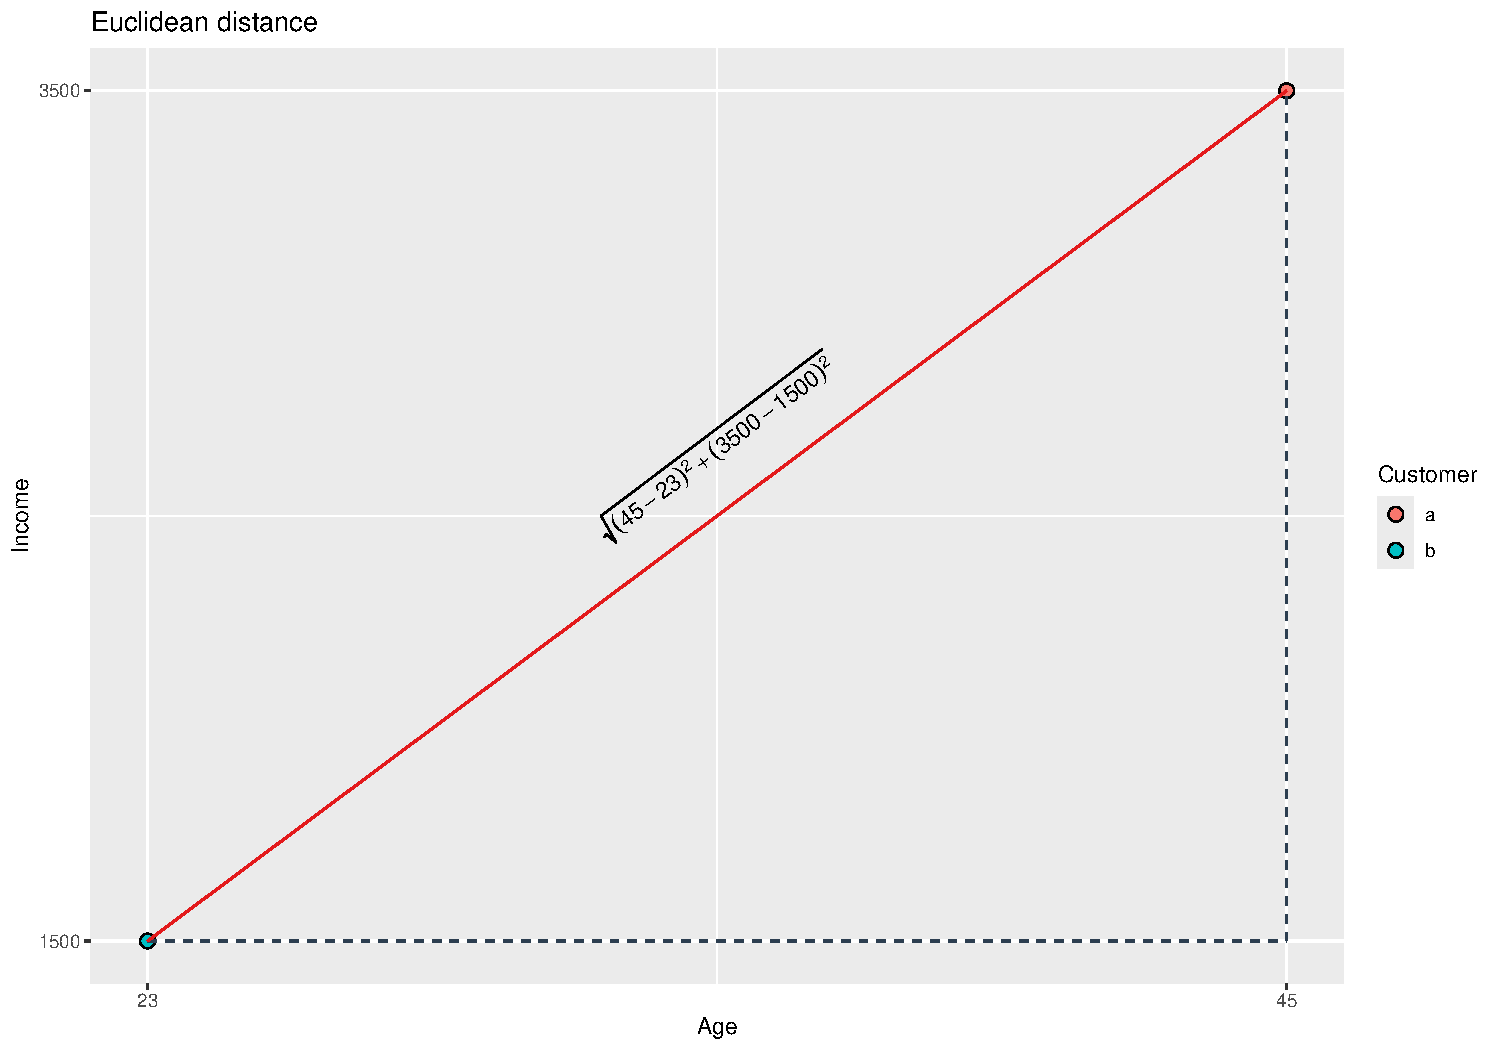
\includegraphics[width=0.6\textwidth,height=\textheight]{011_segmentation_clustering_files/figure-beamer/unnamed-chunk-6-1.pdf}
\end{center}
\end{frame}

\begin{frame}[fragile]{}
\phantomsection\label{section-11}
\begin{itemize}
\tightlist
\item
  Using R
\end{itemize}

\tiny

\begin{Shaded}
\begin{Highlighting}[]
\NormalTok{customers }\OtherTok{\textless{}{-}} \FunctionTok{tibble}\NormalTok{(}\AttributeTok{Customer =} \FunctionTok{c}\NormalTok{(}\StringTok{"a"}\NormalTok{, }\StringTok{"b"}\NormalTok{),}
                    \AttributeTok{Age =} \FunctionTok{c}\NormalTok{(}\DecValTok{45}\NormalTok{, }\DecValTok{23}\NormalTok{),}
                    \AttributeTok{Income =} \FunctionTok{c}\NormalTok{(}\DecValTok{3500}\NormalTok{, }\DecValTok{1500}\NormalTok{))}
\NormalTok{customers}
\end{Highlighting}
\end{Shaded}

\begin{verbatim}
# A tibble: 2 x 3
  Customer   Age Income
  <chr>    <dbl>  <dbl>
1 a           45   3500
2 b           23   1500
\end{verbatim}

\begin{Shaded}
\begin{Highlighting}[]
\FunctionTok{library}\NormalTok{(cluster)}
\NormalTok{customers }\SpecialCharTok{|\textgreater{}} 
  \FunctionTok{select}\NormalTok{(}\SpecialCharTok{{-}}\NormalTok{Customer) }\SpecialCharTok{|\textgreater{}} 
  \FunctionTok{daisy}\NormalTok{(}\AttributeTok{metric =} \StringTok{"euclidean"}\NormalTok{)}
\end{Highlighting}
\end{Shaded}

\begin{verbatim}
Dissimilarities :
         1
2 2000.121

Metric :  euclidean 
Number of objects : 2
\end{verbatim}
\end{frame}

\begin{frame}{}
\phantomsection\label{section-12}
\begin{itemize}
\item
  \textbf{Gower distance}: it can be used for categorical, numerical
  data and missing values

  \begin{itemize}
  \tightlist
  \item
    \(x = (x_1, x_2, \ldots, x_n)\)
  \item
    \(y = (y_1, y_2, \ldots, y_n)\)
  \end{itemize}
\end{itemize}

\tiny

\[\begin{split}
  d(x,y) & = \left[ \frac{w_1\delta_{x_1y_1}^k}{\sum_{k=1}^n w_k\delta_{x_iy_i}^k}\right] d_{x_1y_1}^1 + \left[ \frac{w_2\delta_{x_2y_2}^k}{\sum_{k=1}^n w_k\delta_{x_iy_i}^k} \right] d_{x_2y_2}^2 + \ldots + \left[ \frac{w_n\delta_{x_ny_n}^k}{\sum_{k=1}^n w_k\delta_{x_iy_i}^k} \right] d_{x_ny_n}^n \\ 
  & = \frac{\sum_{k=1}^n w_k \delta_{x_iy_i}^kd_{x_iy_i}^k}{\sum_{k=1}^n w_k\delta_{x_iy_i}^k}
  \end{split}\]

\scriptsize

Where:

\footnotesize

\[w_k \in \mathbb{R} \text{ for } k = 1, 2, \ldots, n\]

\[\sum_{k=1}^n w_k\delta_{x_iy_i}^k = w_1\delta_{x_1y_1}^1 + w_2\delta_{x_2y_2}^2 + \ldots + w_n\delta_{x_ny_n}^n\]
\end{frame}

\begin{frame}{}
\phantomsection\label{section-13}
\begin{itemize}
\item
  \textbf{Gower distance}: it can be used for categorical, numerical
  data and missing values

  \begin{itemize}
  \tightlist
  \item
    \(x = (x_1, x_2, \ldots, x_n)\)
  \item
    \(y = (y_1, y_2, \ldots, y_n)\)
  \end{itemize}
\end{itemize}

\[d(x,y) = \frac{\sum_{k=1}^n w_k \delta_{x_ky_k}^kd_{x_ky_k}^k}{\sum_{k=1}^n w_k\delta_{x_ky_k}^k}\]

\scriptsize

Where\footnote<.->{See (\citeproc{ref-kaufman_finding_1990}{Kaufman and
  Rousseeuw 1990, 25--27}) for a definition of \textbf{asymmetric binary
  variable}}:

\footnotesize

\[\delta_{x_ky_k}^k = 
  \begin{cases}
   0 & \text{if } x_k \text{ or } y_k \text{ is a missing value}\\
   0 & \text{if } x_k, y_k \text{ represent an  asymmetric binary variable and } x_k = y_k = 0 \\
   1 & \text{otherwise}
  \end{cases}\]
\end{frame}

\begin{frame}{}
\phantomsection\label{section-14}
\begin{itemize}
\item
  \textbf{Gower distance}: it can be used for categorical, numerical
  data and missing values

  \begin{itemize}
  \tightlist
  \item
    \(x = (x_1, x_2, \ldots, x_n)\)
  \item
    \(y = (y_1, y_2, \ldots, y_n)\)
  \end{itemize}
\end{itemize}

\[d(x,y) = \frac{\sum_{k=1}^n w_k \delta_{x_ky_k}^kd_{x_ky_k}^k}{\sum_{k=1}^n w_k\delta_{x_ky_k}^k}\]

\scriptsize

Where:

\tiny

\[d_{x_ky_k}^k = 
  \begin{cases}
   0 & \text{if } x_k, y_k \text{ represent a nominal or binary variable and } x_k = y_k \\
   1 & \text{if } x_k, y_k \text{ represent a nominal or binary variable and } x_k \neq y_k \\
   \frac{\left| x_k - y_k \right|}{max(x_k, y_k) - min(x_k, y_k)} & \text{otherwise}
  \end{cases}\]

\scriptsize

If \(x_k, y_k\) represent an ordinal variable they are replaced by their
integer codes. For example if \(x_k \precsim y_k\) then \(1\) is
assigned to \(x_k\) and \(2\) is assigned to \(y_k\)
\end{frame}

\begin{frame}{}
\phantomsection\label{section-15}
\begin{itemize}
\item
  An example:

  \begin{itemize}
  \item
    2 customers characteristic by sex (nominal), income (numerical),
    satisfaction (ordinal with levels
    \(Low \precsim Medium \precsim High\)) and age (with a missing value
    \((NA)\))

    \begin{itemize}
    \tightlist
    \item
      \(a = (Female, 3500, Medium, 45)\)
    \item
      \(b = (Male, 1500, High, NA)\)
    \end{itemize}
  \end{itemize}
\item
  Manual calculation:

  \begin{itemize}
  \item
    In R \(w_k = 1\) for every \(k\) as a default value where in this
    example \(k = 1, 2, 3, 4\)
  \item
    \(\sum_{k=1}^4 w_k\delta_{x_ky_k}^k = 1*1 + 1*1 + 1*1 + 1*0 = 1 + 1 + 1 + 0 = 3\)
  \item
    \(\sum_{k=1}^4 w_k \delta_{x_ky_k}^kd_{x_ky_k}^k = 1*1 + 1*\frac{\left| 3500 - 1500 \right|}{3500 - 1500} + 1*\frac{\left| 2 - 3 \right|}{3 - 2} + 0 = 3\)
  \item
    \(d(x,y) = \frac{\sum_{k=1}^4 w_k \delta_{x_ky_k}^kd_{x_ky_k}^k}{\sum_{k=1}^4 w_k\delta_{x_ky_k}^k} = \frac{3}{3} = 1\)
  \end{itemize}
\end{itemize}
\end{frame}

\begin{frame}[fragile]{}
\phantomsection\label{section-16}
\begin{itemize}
\item
  \textbf{Gower distance} range:

  \begin{itemize}
  \tightlist
  \item
    \(d(x,y) \in [0,1]\)
  \item
    If \(d(x,y) \longrightarrow 0\) is more similar
  \item
    If \(d(x,y) \longrightarrow 1\) is more dissimilar
  \end{itemize}
\item
  Using R
\end{itemize}

\tiny

\begin{Shaded}
\begin{Highlighting}[]
\NormalTok{customers2 }\OtherTok{\textless{}{-}} \FunctionTok{tibble}\NormalTok{(}\AttributeTok{Customer =} \FunctionTok{c}\NormalTok{(}\StringTok{"a"}\NormalTok{, }\StringTok{"b"}\NormalTok{),}
                     \AttributeTok{Sex =} \FunctionTok{c}\NormalTok{(}\StringTok{"Female"}\NormalTok{, }\StringTok{"Male"}\NormalTok{),}
                     \AttributeTok{Income =} \FunctionTok{c}\NormalTok{(}\DecValTok{3500}\NormalTok{, }\DecValTok{1500}\NormalTok{),}
                     \AttributeTok{Satisfaction =} \FunctionTok{c}\NormalTok{(}\StringTok{"Medium"}\NormalTok{, }\StringTok{"High"}\NormalTok{),}
                     \AttributeTok{Age =} \FunctionTok{c}\NormalTok{(}\DecValTok{45}\NormalTok{, }\ConstantTok{NA}\NormalTok{)) }\SpecialCharTok{|\textgreater{}} 
  \FunctionTok{mutate}\NormalTok{(}\AttributeTok{Sex =} \FunctionTok{factor}\NormalTok{(}\AttributeTok{x =}\NormalTok{ Sex, }
                      \AttributeTok{ordered =} \ConstantTok{FALSE}\NormalTok{),}
         \AttributeTok{Satisfaction =} \FunctionTok{factor}\NormalTok{(}\AttributeTok{x =}\NormalTok{ Satisfaction, }
                               \AttributeTok{levels =} \FunctionTok{c}\NormalTok{(}\StringTok{"Low"}\NormalTok{, }\StringTok{"Medium"}\NormalTok{, }\StringTok{"High"}\NormalTok{),}
                               \AttributeTok{ordered =} \ConstantTok{TRUE}\NormalTok{))}
\NormalTok{customers2}
\end{Highlighting}
\end{Shaded}

\begin{verbatim}
# A tibble: 2 x 5
  Customer Sex    Income Satisfaction   Age
  <chr>    <fct>   <dbl> <ord>        <dbl>
1 a        Female   3500 Medium          45
2 b        Male     1500 High            NA
\end{verbatim}
\end{frame}

\begin{frame}[fragile]{}
\phantomsection\label{section-17}
\begin{itemize}
\tightlist
\item
  Using R
\end{itemize}

\tiny

\begin{Shaded}
\begin{Highlighting}[]
\NormalTok{customers2 }\SpecialCharTok{|\textgreater{}}
  \FunctionTok{select}\NormalTok{(}\SpecialCharTok{{-}}\NormalTok{Customer) }\SpecialCharTok{|\textgreater{}}
  \FunctionTok{daisy}\NormalTok{(}\AttributeTok{metric =} \StringTok{"gower"}\NormalTok{)}
\end{Highlighting}
\end{Shaded}

\begin{verbatim}
Dissimilarities :
  1
2 1

Metric :  mixed ;  Types = N, I, O, I 
Number of objects : 2
\end{verbatim}

\normalsize

\begin{itemize}
\item
  In this case:

  \begin{itemize}
  \item
    \texttt{Metric:\ mixed} because it includes categorical and
    numerical data
  \item
    For \texttt{Types\ =\ N,\ I,\ O,\ I} check out
    \texttt{?cluster::dissimilarity.object}\footnote<.->{See
      (\citeproc{ref-stevens_theory_1946}{Stevens 1946}) and
      \href{https://en.wikipedia.org/wiki/Level_of_measurement}{Level of
      measurement}}

    \begin{itemize}
    \tightlist
    \item
      \texttt{N}: Nominal (factor)
    \item
      \texttt{I}: Interval scaled (numeric)
    \item
      \texttt{O}: Ordinal (ordered factor)
    \end{itemize}
  \end{itemize}
\end{itemize}
\end{frame}

\begin{frame}[fragile]{}
\phantomsection\label{section-18}
\begin{itemize}
\tightlist
\item
  Using R
\end{itemize}

\tiny

\begin{Shaded}
\begin{Highlighting}[]
\NormalTok{customers2 }\SpecialCharTok{|\textgreater{}}
  \FunctionTok{select}\NormalTok{(}\SpecialCharTok{{-}}\NormalTok{Customer) }\SpecialCharTok{|\textgreater{}}
  \FunctionTok{daisy}\NormalTok{(}\AttributeTok{metric =} \StringTok{"gower"}\NormalTok{)}
\end{Highlighting}
\end{Shaded}

\begin{verbatim}
Dissimilarities :
  1
2 1

Metric :  mixed ;  Types = N, I, O, I 
Number of objects : 2
\end{verbatim}

\normalsize

\begin{itemize}
\item
  In this case:

  \begin{itemize}
  \item
    \texttt{Number\ of\ objects\ :\ 2}

    \begin{itemize}
    \tightlist
    \item
      There are 2 observations that correspond to customers \textbf{a}
      and \textbf{b}: \(a = (Female, 3500, Medium, 45)\) and
      \(b = (Male, 1500, High, NA)\)
    \end{itemize}
  \end{itemize}
\end{itemize}
\end{frame}

\begin{frame}[fragile]{}
\phantomsection\label{section-19}
\begin{itemize}
\item
  The original dissimilarity matrix is of dimension \(300 \times 300\)

  \begin{itemize}
  \item
    Showing only the relation between the first \(5\) observations
  \item
    The position \((i,j)\) means the dissimilarity between the
    observations \(i\) and \(j\)

    \begin{itemize}
    \tightlist
    \item
      For example \((4, 3)\), which is equal to \(0.425\), is the
      dissimilarity between the observations \(4\) and \(3\)
    \end{itemize}
  \end{itemize}
\end{itemize}

\tiny

\begin{Shaded}
\begin{Highlighting}[]
\NormalTok{segmentation\_dist }\OtherTok{\textless{}{-}}\NormalTok{ segmentation }\SpecialCharTok{|\textgreater{}} 
  \FunctionTok{daisy}\NormalTok{(}\AttributeTok{metric =} \StringTok{"gower"}\NormalTok{)}

\NormalTok{segmentation\_dist }\SpecialCharTok{|\textgreater{}} 
  \FunctionTok{as.matrix}\NormalTok{() }\SpecialCharTok{|\textgreater{}} 
  \FunctionTok{as\_tibble}\NormalTok{() }\SpecialCharTok{|\textgreater{}} 
  \FunctionTok{select}\NormalTok{(}\StringTok{\textasciigrave{}}\AttributeTok{1}\StringTok{\textasciigrave{}}\SpecialCharTok{:}\StringTok{\textasciigrave{}}\AttributeTok{5}\StringTok{\textasciigrave{}}\NormalTok{) }\SpecialCharTok{|\textgreater{}} 
  \FunctionTok{slice}\NormalTok{(}\DecValTok{1}\SpecialCharTok{:}\DecValTok{5}\NormalTok{)}
\end{Highlighting}
\end{Shaded}

\begin{verbatim}
# A tibble: 5 x 5
    `1`    `2`    `3`   `4`   `5`
  <dbl>  <dbl>  <dbl> <dbl> <dbl>
1 0     0.253  0.233  0.262 0.416
2 0.253 0      0.0680 0.413 0.301
3 0.233 0.0680 0      0.425 0.293
4 0.262 0.413  0.425  0     0.227
5 0.416 0.301  0.293  0.227 0    
\end{verbatim}
\end{frame}

\begin{frame}[fragile]{}
\phantomsection\label{section-20}
\tiny

\begin{Shaded}
\begin{Highlighting}[]
\NormalTok{customers3 }\OtherTok{\textless{}{-}} \FunctionTok{tibble}\NormalTok{(}\AttributeTok{Customer =} \FunctionTok{c}\NormalTok{(}\StringTok{"a"}\NormalTok{, }\StringTok{"b"}\NormalTok{, }\StringTok{"c"}\NormalTok{, }\StringTok{"d"}\NormalTok{, }\StringTok{"e"}\NormalTok{),}
                     \AttributeTok{Sex =} \FunctionTok{c}\NormalTok{(}\StringTok{"Female"}\NormalTok{, }\StringTok{"Male"}\NormalTok{, }\StringTok{"Female"}\NormalTok{, }\StringTok{"Female"}\NormalTok{, }\StringTok{"Male"}\NormalTok{),}
                     \AttributeTok{Income =} \FunctionTok{c}\NormalTok{(}\DecValTok{3500}\NormalTok{, }\DecValTok{1500}\NormalTok{, }\DecValTok{200}\NormalTok{, }\DecValTok{450}\NormalTok{, }\DecValTok{5000}\NormalTok{),}
                     \AttributeTok{Satisfaction =} \FunctionTok{c}\NormalTok{(}\StringTok{"Medium"}\NormalTok{, }\StringTok{"High"}\NormalTok{, }\StringTok{"Low"}\NormalTok{, }\StringTok{"Low"}\NormalTok{, }\StringTok{"Medium"}\NormalTok{),}
                     \AttributeTok{Age =} \FunctionTok{c}\NormalTok{(}\DecValTok{45}\NormalTok{, }\ConstantTok{NA}\NormalTok{, }\DecValTok{34}\NormalTok{, }\DecValTok{23}\NormalTok{, }\DecValTok{55}\NormalTok{)) }\SpecialCharTok{|\textgreater{}} 
  \FunctionTok{mutate}\NormalTok{(}\AttributeTok{Sex =} \FunctionTok{factor}\NormalTok{(}\AttributeTok{x =}\NormalTok{ Sex, }
                      \AttributeTok{ordered =} \ConstantTok{FALSE}\NormalTok{),}
         \AttributeTok{Satisfaction =} \FunctionTok{factor}\NormalTok{(}\AttributeTok{x =}\NormalTok{ Satisfaction, }
                               \AttributeTok{levels =} \FunctionTok{c}\NormalTok{(}\StringTok{"Low"}\NormalTok{, }\StringTok{"Medium"}\NormalTok{, }\StringTok{"High"}\NormalTok{),}
                               \AttributeTok{ordered =} \ConstantTok{TRUE}\NormalTok{))}

\NormalTok{customers3}
\end{Highlighting}
\end{Shaded}

\begin{verbatim}
# A tibble: 5 x 5
  Customer Sex    Income Satisfaction   Age
  <chr>    <fct>   <dbl> <ord>        <dbl>
1 a        Female   3500 Medium          45
2 b        Male     1500 High            NA
3 c        Female    200 Low             34
4 d        Female    450 Low             23
5 e        Male     5000 Medium          55
\end{verbatim}
\end{frame}

\begin{frame}[fragile]{}
\phantomsection\label{section-21}
\begin{itemize}
\item
  Hierarchical clustering

  \begin{itemize}
  \tightlist
  \item
    \textbf{Method}: Complete Linkage Clustering
  \end{itemize}
\end{itemize}

\tiny

\begin{Shaded}
\begin{Highlighting}[]
\NormalTok{customers3\_dist }\OtherTok{\textless{}{-}} \FunctionTok{daisy}\NormalTok{(}\AttributeTok{x =} \FunctionTok{select}\NormalTok{(customers3, }\SpecialCharTok{{-}}\NormalTok{Customer),}
                        \AttributeTok{metric =} \StringTok{"gower"}\NormalTok{)}

\NormalTok{customers3\_dist}
\end{Highlighting}
\end{Shaded}

\begin{verbatim}
Dissimilarities :
           1          2          3          4
2 0.63888889                                 
3 0.38281250 0.75694444                      
4 0.45572917 0.73958333 0.09895833           
5 0.40625000 0.40972222 0.78906250 0.86197917

Metric :  mixed ;  Types = N, I, O, I 
Number of objects : 5
\end{verbatim}

\begin{Shaded}
\begin{Highlighting}[]
\NormalTok{customers3\_hc }\OtherTok{\textless{}{-}} \FunctionTok{hclust}\NormalTok{(}\AttributeTok{d =}\NormalTok{ customers3\_dist, }
                        \AttributeTok{method =} \StringTok{"complete"}\NormalTok{)}

\NormalTok{customers3\_hc}
\end{Highlighting}
\end{Shaded}

\begin{verbatim}

Call:
hclust(d = customers3_dist, method = "complete")

Cluster method   : complete 
Number of objects: 5 
\end{verbatim}
\end{frame}

\begin{frame}[fragile]{}
\phantomsection\label{section-22}
\begin{itemize}
\item
  Hierarchical clustering

  \begin{itemize}
  \tightlist
  \item
    \textbf{Method}: Complete Linkage Clustering
  \end{itemize}
\end{itemize}

\tiny

\begin{Shaded}
\begin{Highlighting}[]
\FunctionTok{plot}\NormalTok{(customers3\_hc)}
\end{Highlighting}
\end{Shaded}

\begin{center}
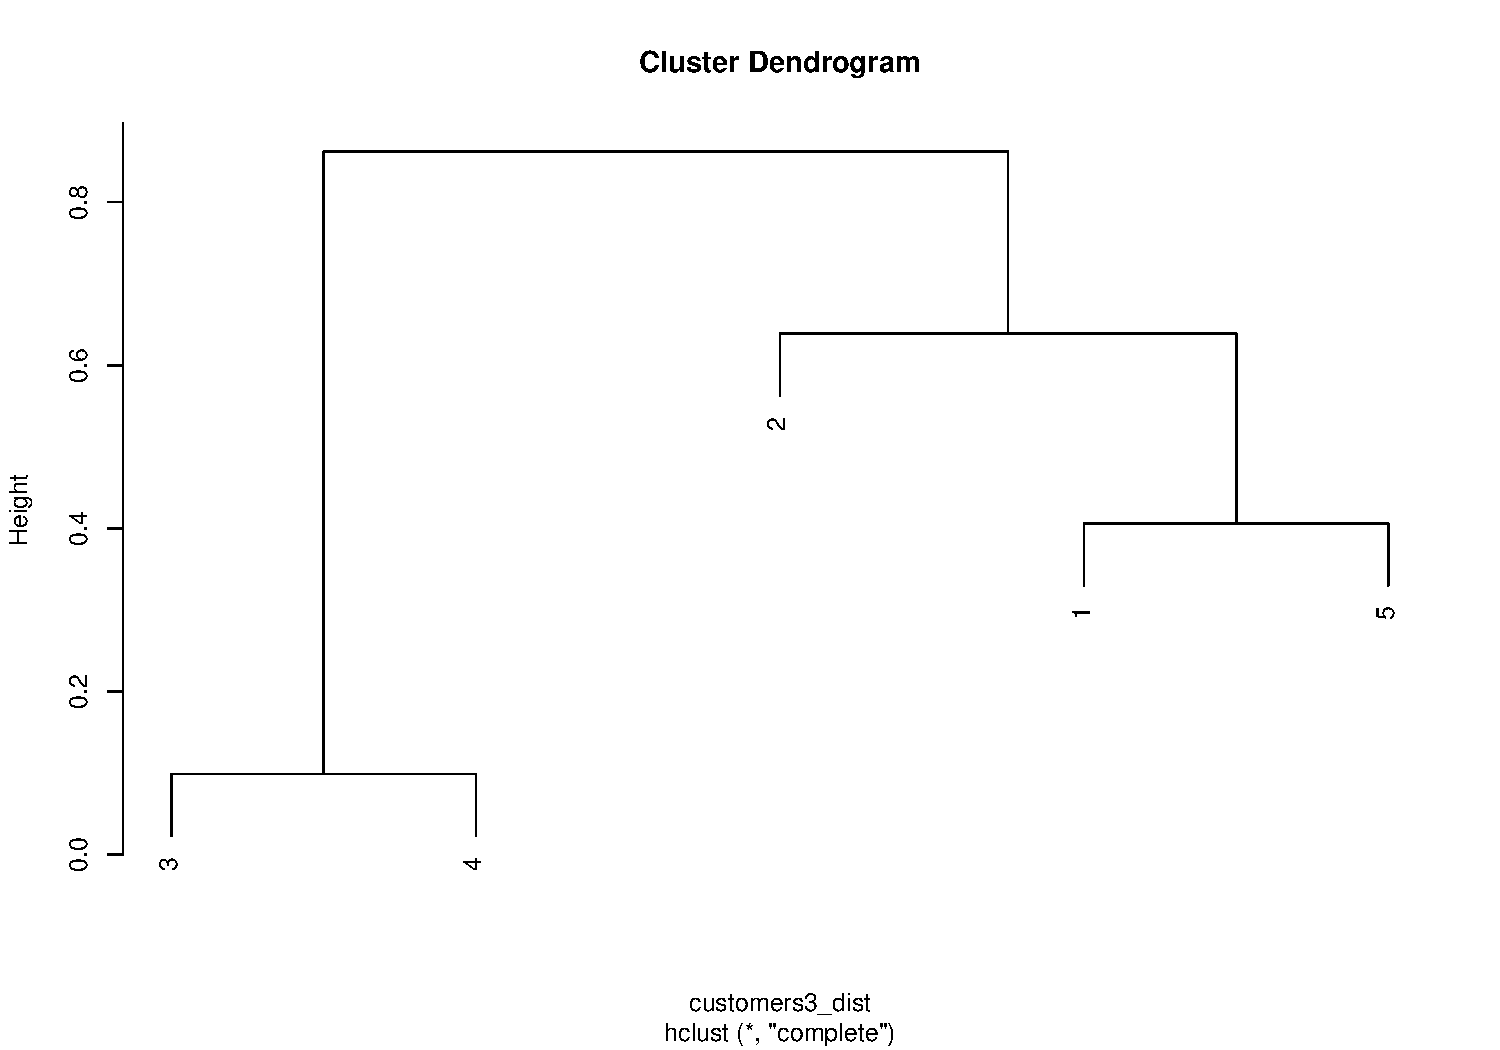
\includegraphics[width=0.6\textwidth,height=\textheight]{011_segmentation_clustering_files/figure-beamer/unnamed-chunk-15-1.pdf}
\end{center}
\end{frame}

\begin{frame}{}
\phantomsection\label{section-23}
\begin{itemize}
\tightlist
\item
  Compare each observation and find the pair that is more similar
\end{itemize}

\begin{table}
\centering
\begin{tabular}[t]{rrrrrr}
\toprule
  & 1 & 2 & 3 & 4 & 5\\
\midrule
1 & 0.0000000 & 0.6388889 & 0.3828125 & 0.4557292 & 0.4062500\\
2 & 0.6388889 & 0.0000000 & 0.75694444 & 0.7395833 & 0.4097222\\
3 & 0.3828125 & 0.7569444 & 0 & 0.0989583 & 0.7890625\\
4 & 0.4557292 & 0.7395833 & \cellcolor[HTML]{2C3E50}{\textcolor{white}{0.09895833}} & 0.0000000 & 0.8619792\\
5 & 0.4062500 & 0.4097222 & 0.7890625 & 0.8619792 & 0.0000000\\
\bottomrule
\end{tabular}
\end{table}
\end{frame}

\begin{frame}{}
\phantomsection\label{section-24}
\begin{itemize}
\item
  Now we have the first cluster that includes the observations \(3\) and
  \(4\): \(C(3,4)\)
\item
  Then we need to create clusters with observations \(1\), \(2\) and
  \(5\) and the cluster \(C(3,4)\)

  \begin{itemize}
  \item
    How we compare a cluster with an observation

    \begin{itemize}
    \tightlist
    \item
      \textbf{Complete Linkage Clustering}: Use the maximum distance
      between an observation and an observation that belongs to the
      cluster
    \end{itemize}
  \end{itemize}
\end{itemize}
\end{frame}

\begin{frame}{}
\phantomsection\label{section-25}
\begin{itemize}
\item
  Compare each observation, including the clusters build, and find the
  pair that is more similar

  \begin{itemize}
  \item
    In our case \(1\), \(2\), \(5\) and \(C(3,4)\)

    \begin{itemize}
    \tightlist
    \item
      The distance between \(1\) and \(C(3,4)\) is \(0.45572917\)\\
    \item
      The distance between \(2\) and \(C(3,4)\) is \(0.7569444\)
    \item
      The distance between \(5\) and \(C(3,4)\) is \(0.8619792\)
    \end{itemize}
  \end{itemize}
\end{itemize}

\begin{table}
\centering
\begin{tabular}[t]{rrrrrr}
\toprule
  & 1 & 2 & 3 & 4 & 5\\
\midrule
1 & 0 & 0.6388889 & 0.3828125 & 0.4557292 & 0.4062500\\
2 & 0.63888889 & 0.0000000 & 0.75694444 & 0.7395833 & 0.4097222\\
3 & 0.3828125 & 0.7569444 & 0 & 0.0989583 & 0.7890625\\
4 & 0.45572917 & 0.7395833 & \cellcolor[HTML]{2C3E50}{\textcolor{white}{0.09895833}} & 0.0000000 & 0.8619792\\
5 & \cellcolor[HTML]{E31A1C}{\textcolor{white}{0.40625}} & 0.4097222 & 0.7890625 & 0.8619792 & 0.0000000\\
\bottomrule
\end{tabular}
\end{table}
\end{frame}

\begin{frame}{}
\phantomsection\label{section-26}
\begin{itemize}
\item
  Now we have the second cluster that includes the observations \(1\)
  and \(5\): \(C(1,5)\)
\item
  Then we need to create clusters with observation \(2\) and clusters
  \(C(3,4)\) and \(C(1,5)\)

  \begin{itemize}
  \item
    How we compare a cluster with another cluster

    \begin{itemize}
    \tightlist
    \item
      \textbf{Complete Linkage Clustering}: Use the maximum distance
      between an observation that belongs to the first cluster and an
      observation that belongs to the second cluster
    \end{itemize}
  \end{itemize}
\end{itemize}
\end{frame}

\begin{frame}{}
\phantomsection\label{section-27}
\begin{itemize}
\item
  Compare each observation, including the clusters build, and find the
  pair that is more similar

  \begin{itemize}
  \item
    In our case \(2\), \(C(3,4)\) and \(C(1,5)\)

    \begin{itemize}
    \tightlist
    \item
      The distance between \(2\) and \(C(3,4)\) is \(0.7569444\)\\
    \item
      The distance between \(2\) and \(C(1,5)\) is \(0.6388889\)
    \end{itemize}
  \end{itemize}
\end{itemize}

\begin{table}
\centering
\begin{tabular}[t]{rrrrrr}
\toprule
  & 1 & 2 & 3 & 4 & 5\\
\midrule
1 & 0 & 0.6388889 & 0.3828125 & 0.4557292 & 0.4062500\\
2 & \cellcolor[HTML]{18BC9C}{\textcolor{white}{0.63888889}} & 0.0000000 & 0.75694444 & 0.7395833 & 0.4097222\\
3 & 0.3828125 & 0.7569444 & 0 & 0.0989583 & 0.7890625\\
4 & 0.45572917 & 0.7395833 & \cellcolor[HTML]{2C3E50}{\textcolor{white}{0.09895833}} & 0.0000000 & 0.8619792\\
5 & \cellcolor[HTML]{E31A1C}{\textcolor{white}{0.40625}} & 0.4097222 & 0.7890625 & 0.8619792 & 0.0000000\\
\bottomrule
\end{tabular}
\end{table}
\end{frame}

\begin{frame}{}
\phantomsection\label{section-28}
\begin{itemize}
\item
  Now we have the third cluster that includes the observation \(2\) and
  the cluster \(C(1,5)\): \(C(2, C(1,5))\)
\item
  Then we need to create clusters with cluster \(C(2, C(1,5))\) and
  cluster \(C(3,4)\)

  \begin{itemize}
  \tightlist
  \item
    This is the cluster that includes all the observations
  \end{itemize}
\end{itemize}
\end{frame}

\begin{frame}{}
\phantomsection\label{section-29}
\begin{itemize}
\item
  Compare each observation, including the clusters build, and find the
  pair that is more similar

  \begin{itemize}
  \item
    In our case \(C(3,4)\) and \(C(2, C(1,5))\)

    \begin{itemize}
    \tightlist
    \item
      The distance between \(C(3,4)\) and \(C(2, C(1,5))\) is
      \(0.86197917\)
    \end{itemize}
  \end{itemize}
\end{itemize}

\begin{table}
\centering
\begin{tabular}[t]{rrrrrr}
\toprule
  & 1 & 2 & 3 & 4 & 5\\
\midrule
1 & 0 & 0.6388889 & 0.3828125 & 0.45572917 & 0.4062500\\
2 & \cellcolor[HTML]{18BC9C}{\textcolor{white}{0.63888889}} & 0.0000000 & 0.75694444 & 0.73958333 & 0.4097222\\
3 & 0.3828125 & 0.7569444 & 0 & 0.09895833 & 0.7890625\\
4 & 0.45572917 & 0.7395833 & \cellcolor[HTML]{2C3E50}{\textcolor{white}{0.09895833}} & 0 & 0.8619792\\
5 & \cellcolor[HTML]{E31A1C}{\textcolor{white}{0.40625}} & 0.4097222 & 0.7890625 & \cellcolor[HTML]{CCBE93}{\textcolor{white}{0.86197917}} & 0.0000000\\
\bottomrule
\end{tabular}
\end{table}

\begin{itemize}
\tightlist
\item
  The heights of the \textbf{Cluster Dendrogram} are: \(0.09895833\),
  \(0.40625\), \(0.63888889\) and \(0.86197917\)
\end{itemize}
\end{frame}

\begin{frame}[fragile]{}
\phantomsection\label{section-30}
\begin{itemize}
\tightlist
\item
  Select a number of clusters, for example: \(2\) clusters
\end{itemize}

\tiny

\begin{Shaded}
\begin{Highlighting}[]
\FunctionTok{plot}\NormalTok{(customers3\_hc)}
\FunctionTok{rect.hclust}\NormalTok{(customers3\_hc, }\AttributeTok{k =} \DecValTok{2}\NormalTok{, }\AttributeTok{border =} \StringTok{"red"}\NormalTok{)}
\end{Highlighting}
\end{Shaded}

\begin{center}
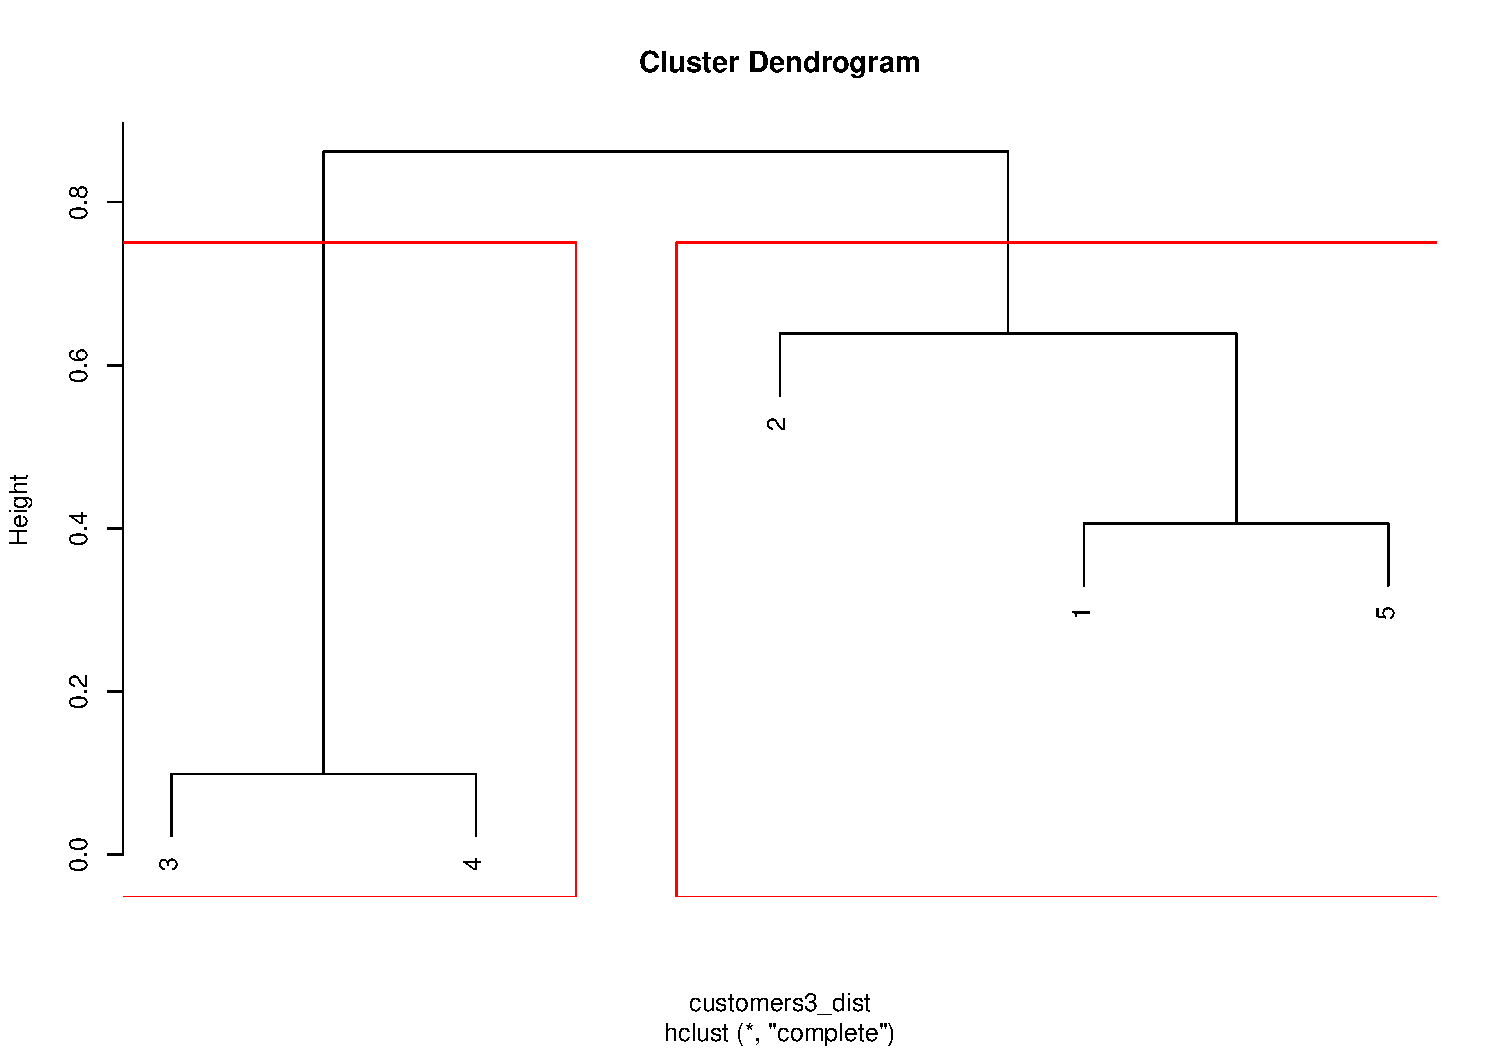
\includegraphics[width=0.6\textwidth,height=\textheight]{011_segmentation_clustering_files/figure-beamer/unnamed-chunk-20-1.pdf}
\end{center}
\end{frame}

\begin{frame}[fragile]{}
\phantomsection\label{section-31}
\begin{itemize}
\tightlist
\item
  Extract clusters and assign them to observations
\end{itemize}

\tiny

\begin{Shaded}
\begin{Highlighting}[]
\NormalTok{customers3\_hc\_clusters }\OtherTok{\textless{}{-}} \FunctionTok{cutree}\NormalTok{(customers3\_hc, }\AttributeTok{k =} \DecValTok{2}\NormalTok{)}
\NormalTok{customers3 }\SpecialCharTok{|\textgreater{}} 
  \FunctionTok{mutate}\NormalTok{(}\AttributeTok{cluster =}\NormalTok{ customers3\_hc\_clusters)}
\end{Highlighting}
\end{Shaded}

\begin{verbatim}
# A tibble: 5 x 6
  Customer Sex    Income Satisfaction   Age cluster
  <chr>    <fct>   <dbl> <ord>        <dbl>   <int>
1 a        Female   3500 Medium          45       1
2 b        Male     1500 High            NA       1
3 c        Female    200 Low             34       2
4 d        Female    450 Low             23       2
5 e        Male     5000 Medium          55       1
\end{verbatim}
\end{frame}

\begin{frame}[fragile]{}
\phantomsection\label{section-32}
\begin{itemize}
\tightlist
\item
  Select a number of clusters, using \texttt{segmentation}, for example:
  \(4\) clusters
\end{itemize}

\tiny

\begin{Shaded}
\begin{Highlighting}[]
\NormalTok{segmentation\_hc }\OtherTok{\textless{}{-}} \FunctionTok{hclust}\NormalTok{(}\AttributeTok{d =}\NormalTok{ segmentation\_dist,}
                          \AttributeTok{method =} \StringTok{"complete"}\NormalTok{)}
\FunctionTok{plot}\NormalTok{(segmentation\_hc)}
\FunctionTok{rect.hclust}\NormalTok{(segmentation\_hc, }\AttributeTok{k =} \DecValTok{4}\NormalTok{, }\AttributeTok{border =} \StringTok{"red"}\NormalTok{)}
\end{Highlighting}
\end{Shaded}

\begin{center}
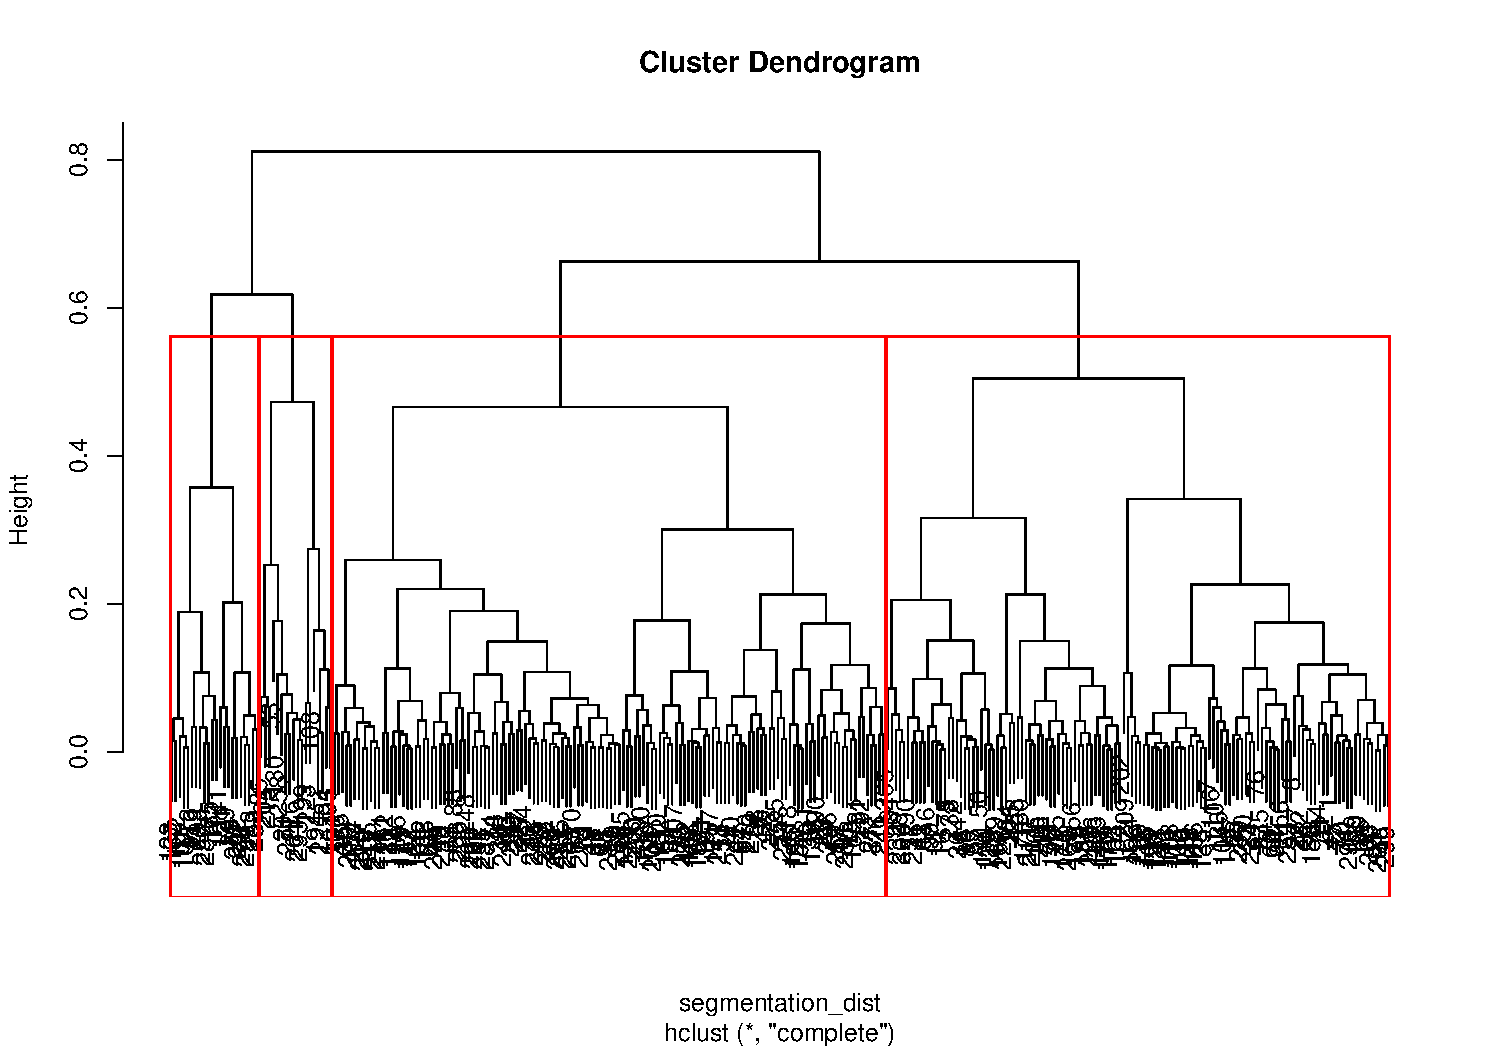
\includegraphics[width=0.6\textwidth,height=\textheight]{011_segmentation_clustering_files/figure-beamer/unnamed-chunk-22-1.pdf}
\end{center}
\end{frame}

\begin{frame}[fragile]{}
\phantomsection\label{section-33}
\begin{itemize}
\tightlist
\item
  Extract clusters and assign them to observations, using
  \texttt{segmentation}
\end{itemize}

\tiny

\begin{Shaded}
\begin{Highlighting}[]
\NormalTok{segmentation\_hc\_clusters }\OtherTok{\textless{}{-}} \FunctionTok{cutree}\NormalTok{(segmentation\_hc, }\AttributeTok{k =} \DecValTok{4}\NormalTok{)}
\NormalTok{segmentation }\SpecialCharTok{|\textgreater{}} 
  \FunctionTok{mutate}\NormalTok{(}\AttributeTok{cluster =}\NormalTok{ segmentation\_hc\_clusters)}
\end{Highlighting}
\end{Shaded}

\begin{verbatim}
# A tibble: 300 x 7
     age gender income  kids ownHome subscribe cluster
   <dbl> <fct>   <dbl> <int> <fct>   <fct>       <int>
 1  47.3 Male   49483.     2 ownNo   subNo           1
 2  31.4 Male   35546.     1 ownYes  subNo           1
 3  43.2 Male   44169.     0 ownYes  subNo           1
 4  37.3 Female 81042.     1 ownNo   subNo           2
 5  41.0 Female 79353.     3 ownYes  subNo           2
 6  43.0 Male   58143.     4 ownYes  subNo           1
 7  37.6 Male   19282.     3 ownNo   subNo           1
 8  28.5 Male   47245.     0 ownNo   subNo           1
 9  44.2 Female 48333.     1 ownNo   subNo           2
10  35.2 Female 52568.     0 ownYes  subNo           2
# i 290 more rows
\end{verbatim}
\end{frame}

\begin{frame}[fragile]{}
\phantomsection\label{section-34}
\begin{itemize}
\tightlist
\item
  K-means clustering example
  (\citeproc{ref-kaufman_finding_1990}{Kaufman and Rousseeuw 1990, 5})
\end{itemize}

\tiny

\begin{Shaded}
\begin{Highlighting}[]
\NormalTok{kaufman\_example }\OtherTok{\textless{}{-}} \FunctionTok{tibble}\NormalTok{(}\AttributeTok{name =} \FunctionTok{c}\NormalTok{(}\StringTok{"Ilan"}\NormalTok{, }\StringTok{"Jacqueline"}\NormalTok{, }\StringTok{"Kim"}\NormalTok{, }\StringTok{"Lieve"}\NormalTok{, }\StringTok{"Leon"}\NormalTok{, }\StringTok{"Peter"}\NormalTok{, }\StringTok{"Talia"}\NormalTok{, }\StringTok{"Tina"}\NormalTok{),}
                          \AttributeTok{weight\_kg =} \FunctionTok{c}\NormalTok{(}\DecValTok{15}\NormalTok{, }\DecValTok{49}\NormalTok{, }\DecValTok{13}\NormalTok{, }\DecValTok{45}\NormalTok{, }\DecValTok{85}\NormalTok{, }\DecValTok{66}\NormalTok{, }\DecValTok{12}\NormalTok{, }\DecValTok{10}\NormalTok{),}
                          \AttributeTok{height\_cm =} \FunctionTok{c}\NormalTok{(}\DecValTok{95}\NormalTok{, }\DecValTok{156}\NormalTok{, }\DecValTok{95}\NormalTok{, }\DecValTok{160}\NormalTok{, }\DecValTok{178}\NormalTok{, }\DecValTok{176}\NormalTok{, }\DecValTok{90}\NormalTok{, }\DecValTok{78}\NormalTok{))}

\NormalTok{kaufman\_example}
\end{Highlighting}
\end{Shaded}

\begin{verbatim}
# A tibble: 8 x 3
  name       weight_kg height_cm
  <chr>          <dbl>     <dbl>
1 Ilan              15        95
2 Jacqueline        49       156
3 Kim               13        95
4 Lieve             45       160
5 Leon              85       178
6 Peter             66       176
7 Talia             12        90
8 Tina              10        78
\end{verbatim}
\end{frame}

\begin{frame}[fragile]{}
\phantomsection\label{section-35}
\begin{itemize}
\tightlist
\item
  K-means clustering example
  (\citeproc{ref-kaufman_finding_1990}{Kaufman and Rousseeuw 1990, 5})
\end{itemize}

\tiny

\begin{Shaded}
\begin{Highlighting}[]
\NormalTok{kaufman\_example }\SpecialCharTok{|\textgreater{}} 
  \FunctionTok{ggplot}\NormalTok{() }\SpecialCharTok{+} 
  \FunctionTok{geom\_point}\NormalTok{(}\FunctionTok{aes}\NormalTok{(}\AttributeTok{x =}\NormalTok{ weight\_kg, }\AttributeTok{y =}\NormalTok{ height\_cm))}
\end{Highlighting}
\end{Shaded}

\begin{center}
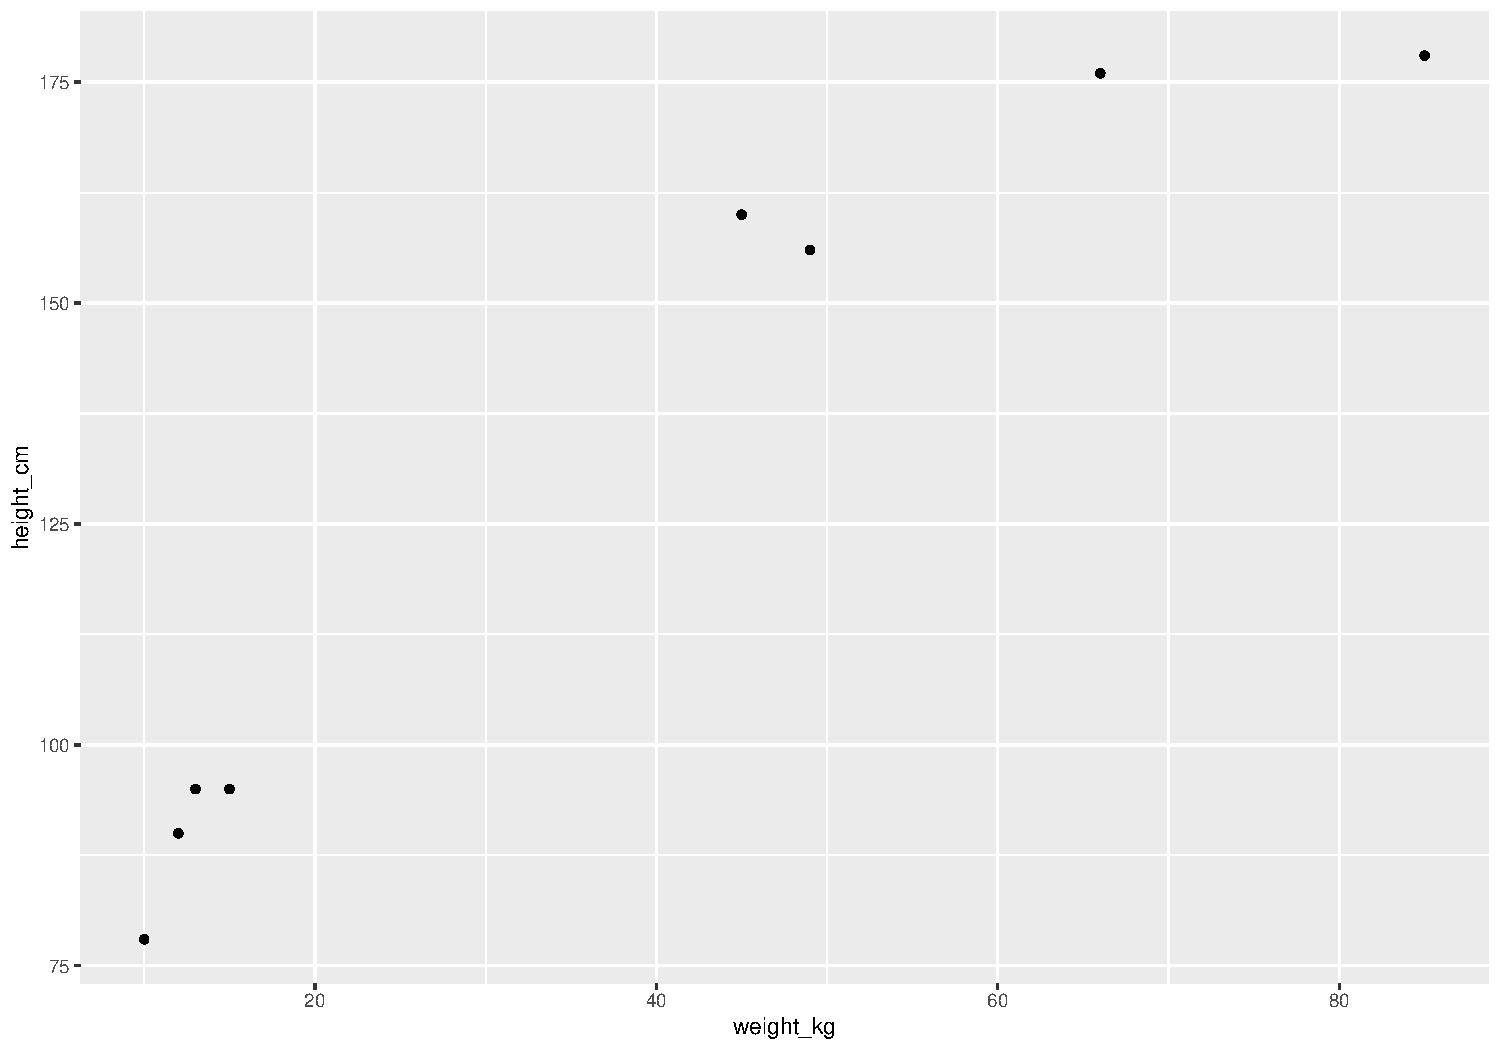
\includegraphics[width=0.6\textwidth,height=\textheight]{011_segmentation_clustering_files/figure-beamer/unnamed-chunk-25-1.pdf}
\end{center}
\end{frame}

\begin{frame}{}
\phantomsection\label{section-36}
\begin{itemize}
\item
  K-means clustering example
  (\citeproc{ref-kaufman_finding_1990}{Kaufman and Rousseeuw 1990, 5})

  \begin{itemize}
  \item
    Applying the
    \href{https://en.wikipedia.org/wiki/K-means_clustering}{\textbf{Lloyd's
    algorithm}}

    \begin{itemize}
    \tightlist
    \item
      Choose \(k\) centers or the computer will choose \(k\) centers at
      random, in our case we choose \(k = 2\)
    \end{itemize}
  \end{itemize}
\end{itemize}

\begin{center}
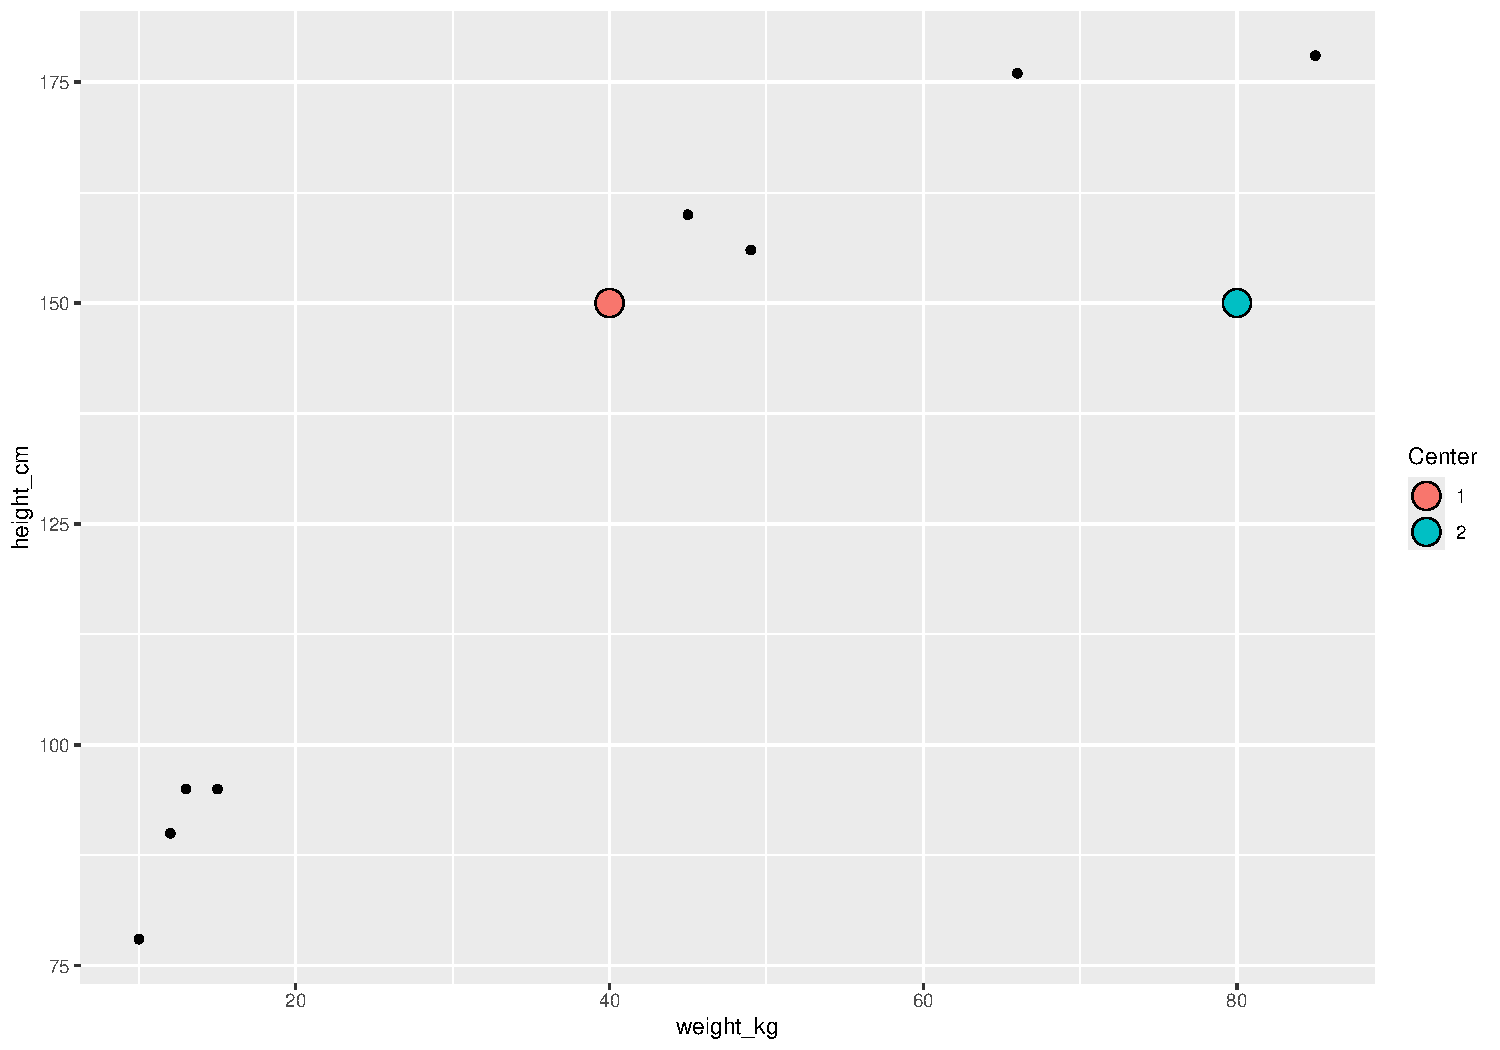
\includegraphics[width=0.6\textwidth,height=\textheight]{011_segmentation_clustering_files/figure-beamer/unnamed-chunk-26-1.pdf}
\end{center}
\end{frame}

\begin{frame}{}
\phantomsection\label{section-37}
\begin{itemize}
\item
  K-means clustering example
  (\citeproc{ref-kaufman_finding_1990}{Kaufman and Rousseeuw 1990, 5})

  \begin{itemize}
  \item
    Applying the
    \href{https://en.wikipedia.org/wiki/K-means_clustering}{\textbf{Lloyd's
    algorithm}}

    \begin{itemize}
    \item
      Calculate the squared euclidean distance for each point to the
      \(k\) centers and assign each point to the nearest center
    \item
      For example for the point \(Ilan = (15, 95)\) the distance to
      \(Center_1 = (40, 150)\) is \((15 - 40)^2 + (95 - 150)^2 = 3650\)
      and the distance to \(Center_2 = (80, 150)\) is
      \((15 - 80)^2 + (95 - 150)^2 = 7250\)
    \item
      Therefore \(Ilan = (15, 95)\) is assigned to \(Center_1\)
    \end{itemize}
  \end{itemize}
\end{itemize}
\end{frame}

\begin{frame}{}
\phantomsection\label{section-38}
\begin{itemize}
\item
  K-means clustering example
  (\citeproc{ref-kaufman_finding_1990}{Kaufman and Rousseeuw 1990, 5})

  \begin{itemize}
  \tightlist
  \item
    Applying the
    \href{https://en.wikipedia.org/wiki/K-means_clustering}{\textbf{Lloyd's
    algorithm}}
  \end{itemize}
\end{itemize}

\begin{center}
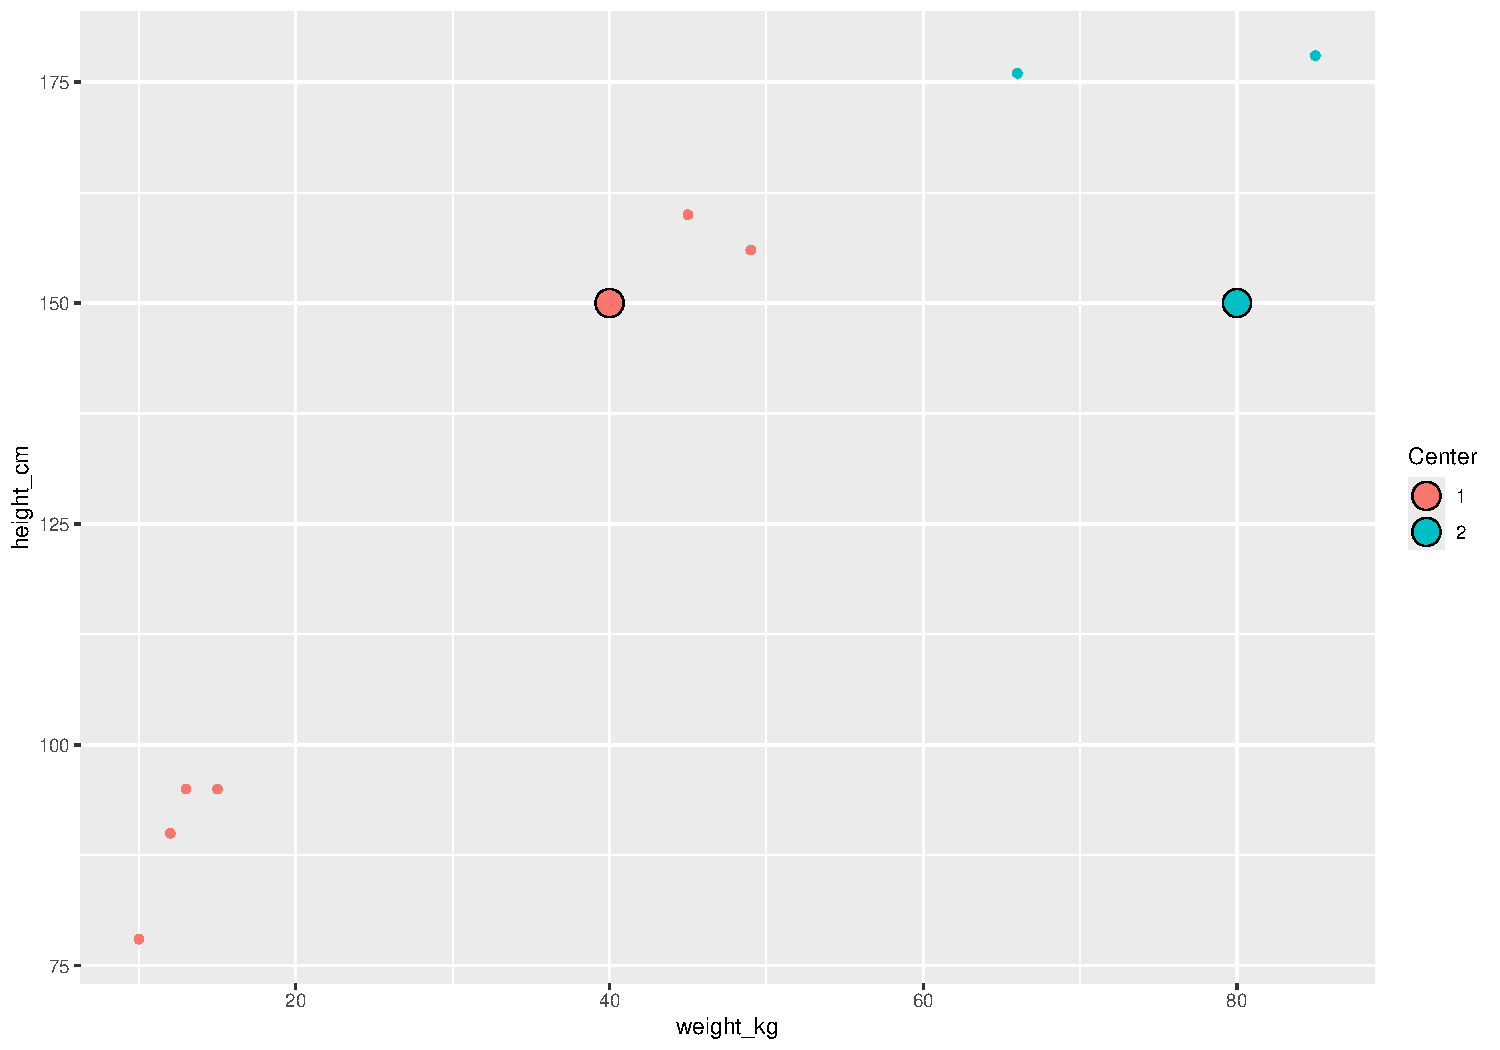
\includegraphics[width=0.6\textwidth,height=\textheight]{011_segmentation_clustering_files/figure-beamer/unnamed-chunk-27-1.pdf}
\end{center}
\end{frame}

\begin{frame}{}
\phantomsection\label{section-39}
\begin{itemize}
\item
  K-means clustering example
  (\citeproc{ref-kaufman_finding_1990}{Kaufman and Rousseeuw 1990, 5})

  \begin{itemize}
  \item
    Applying the
    \href{https://en.wikipedia.org/wiki/K-means_clustering}{\textbf{Lloyd's
    algorithm}}

    \begin{itemize}
    \item
      Now calculate new centers using the assigned points by using the
      mean
    \item
      For example for the new \(Center_1\) the new position will be
      \(x = \frac{15 + 49 + 13 + 45 + 12 + 10}{6} = 24\) and
      \(y = \frac{95 + 156 + 95 + 160 + 90 + 78}{6} \approx 112.33\)
    \item
      Therefore we update as \(Center_1 \approx (24, 112.33)\)
    \end{itemize}
  \end{itemize}
\end{itemize}
\end{frame}

\begin{frame}{}
\phantomsection\label{section-40}
\begin{itemize}
\item
  K-means clustering example
  (\citeproc{ref-kaufman_finding_1990}{Kaufman and Rousseeuw 1990, 5})

  \begin{itemize}
  \tightlist
  \item
    Applying the
    \href{https://en.wikipedia.org/wiki/K-means_clustering}{\textbf{Lloyd's
    algorithm}}
  \end{itemize}
\end{itemize}

\begin{center}
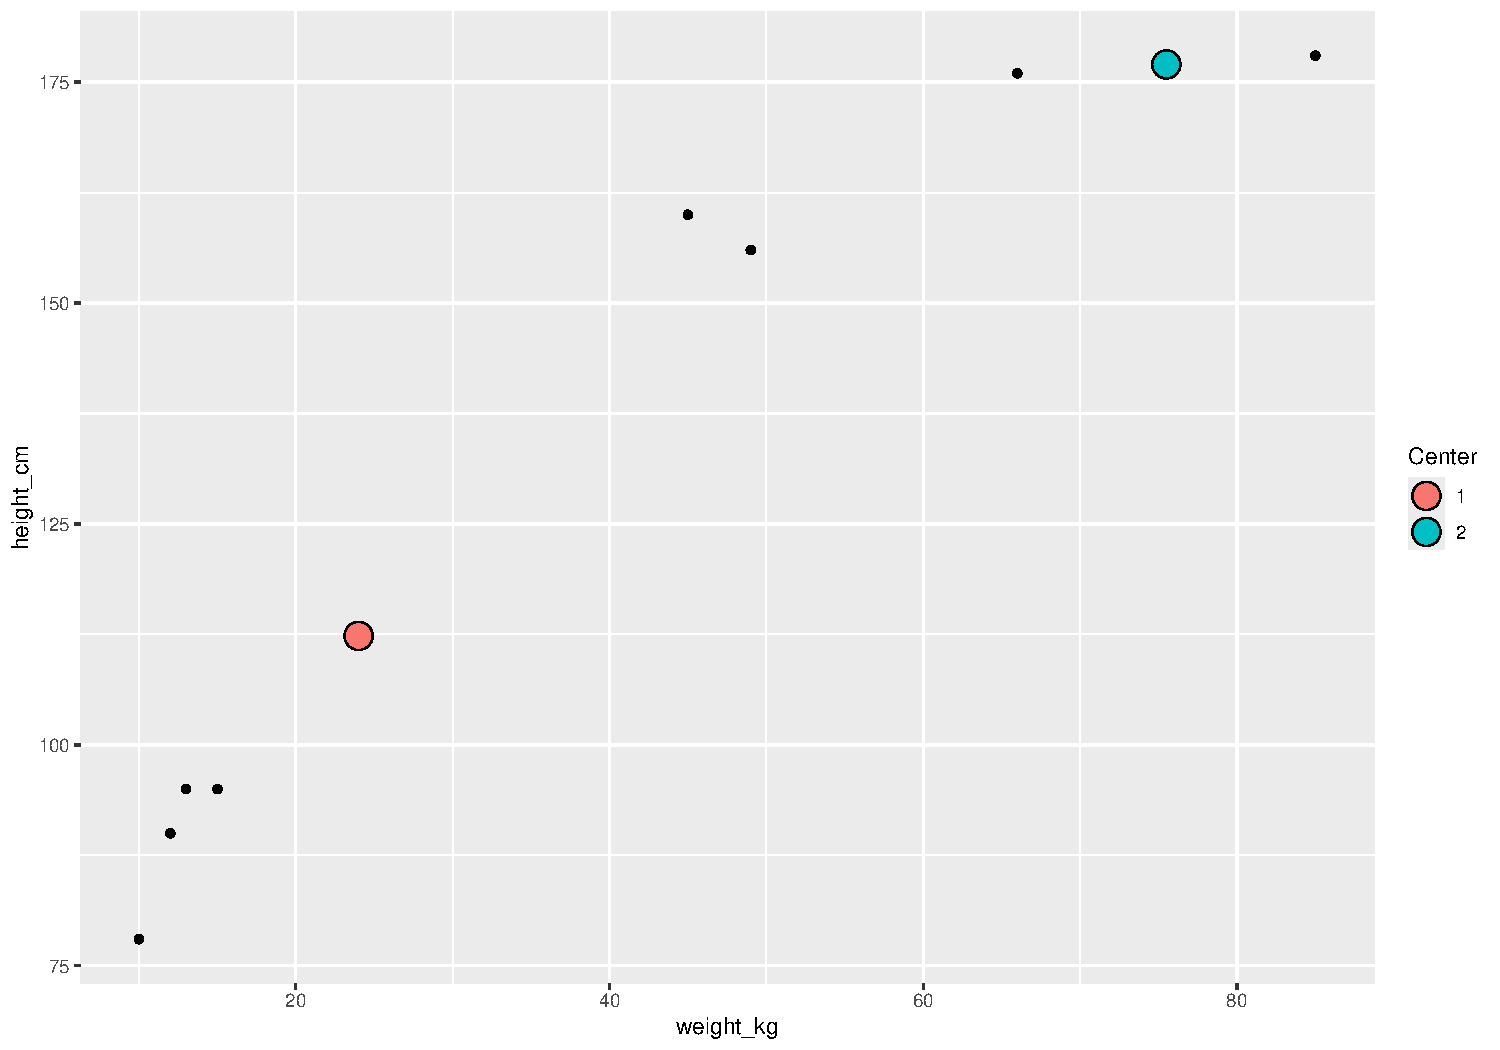
\includegraphics[width=0.6\textwidth,height=\textheight]{011_segmentation_clustering_files/figure-beamer/unnamed-chunk-28-1.pdf}
\end{center}
\end{frame}

\begin{frame}{}
\phantomsection\label{section-41}
\begin{itemize}
\item
  K-means clustering example
  (\citeproc{ref-kaufman_finding_1990}{Kaufman and Rousseeuw 1990, 5})

  \begin{itemize}
  \item
    Applying the
    \href{https://en.wikipedia.org/wiki/K-means_clustering}{\textbf{Lloyd's
    algorithm}}
  \item
    Repeat the process by calculating the squared euclidean distance for
    each point to the new \(k\) centers and assign each point to the
    nearest center
  \end{itemize}
\end{itemize}

\begin{center}
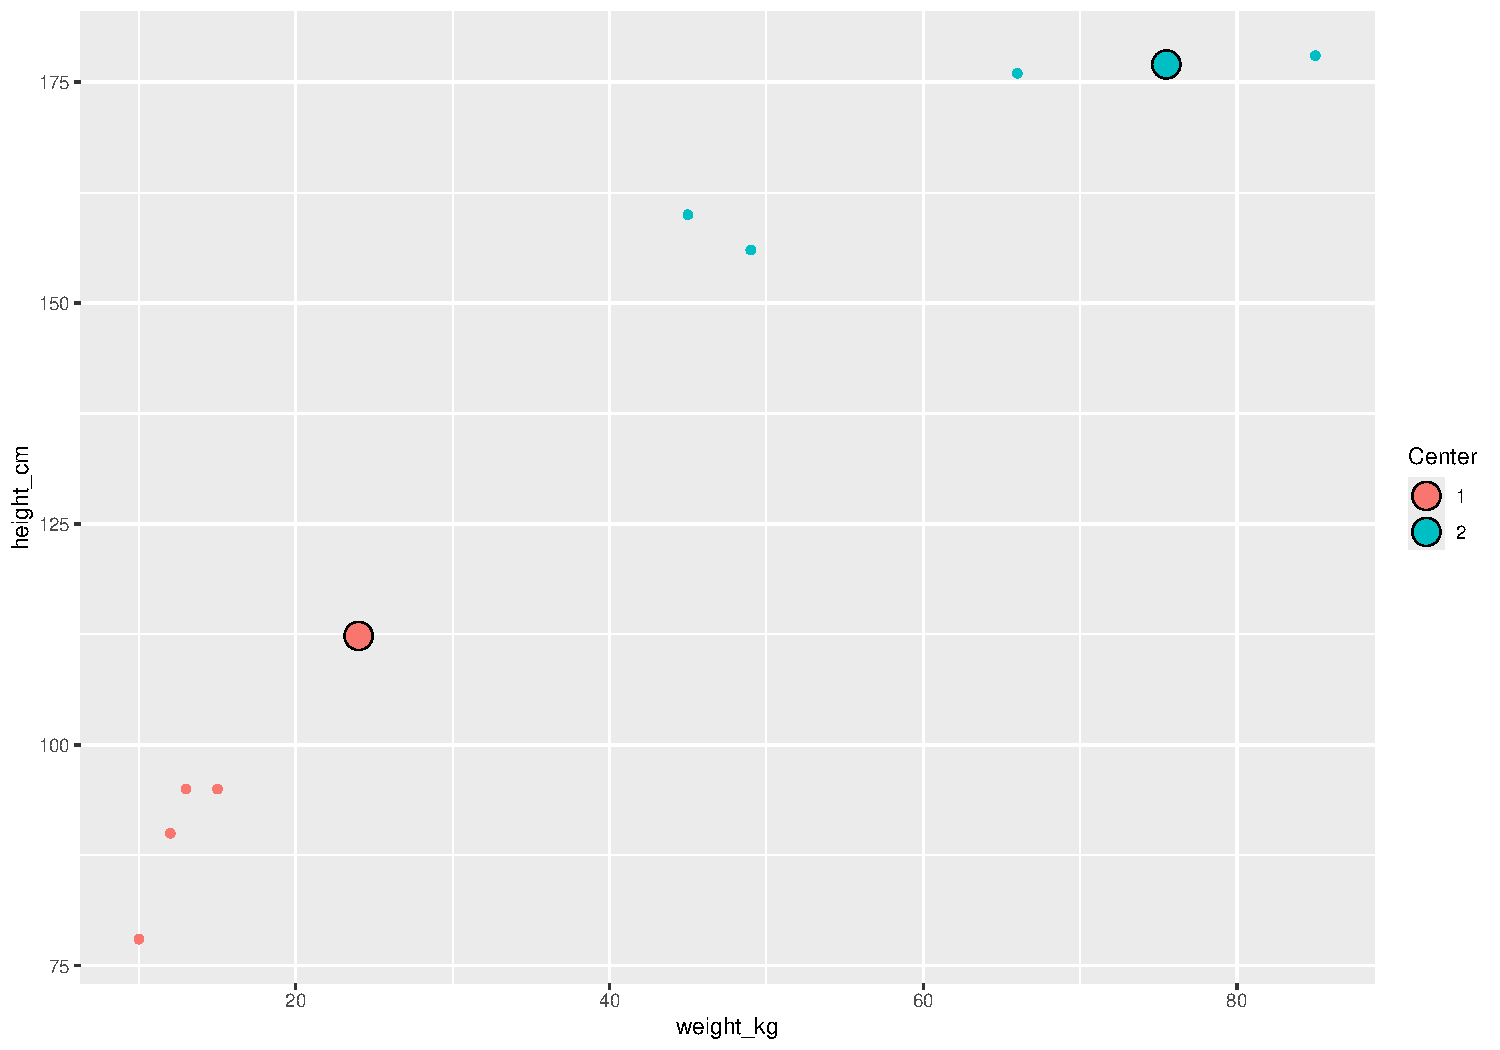
\includegraphics[width=0.6\textwidth,height=\textheight]{011_segmentation_clustering_files/figure-beamer/unnamed-chunk-29-1.pdf}
\end{center}
\end{frame}

\begin{frame}{}
\phantomsection\label{section-42}
\begin{itemize}
\item
  K-means clustering example
  (\citeproc{ref-kaufman_finding_1990}{Kaufman and Rousseeuw 1990, 5})

  \begin{itemize}
  \item
    Applying the
    \href{https://en.wikipedia.org/wiki/K-means_clustering}{\textbf{Lloyd's
    algorithm}}
  \item
    Repeat the process until the \(k\) centers don't change and assign
    each point to the nearest final center
  \end{itemize}
\end{itemize}

\begin{center}
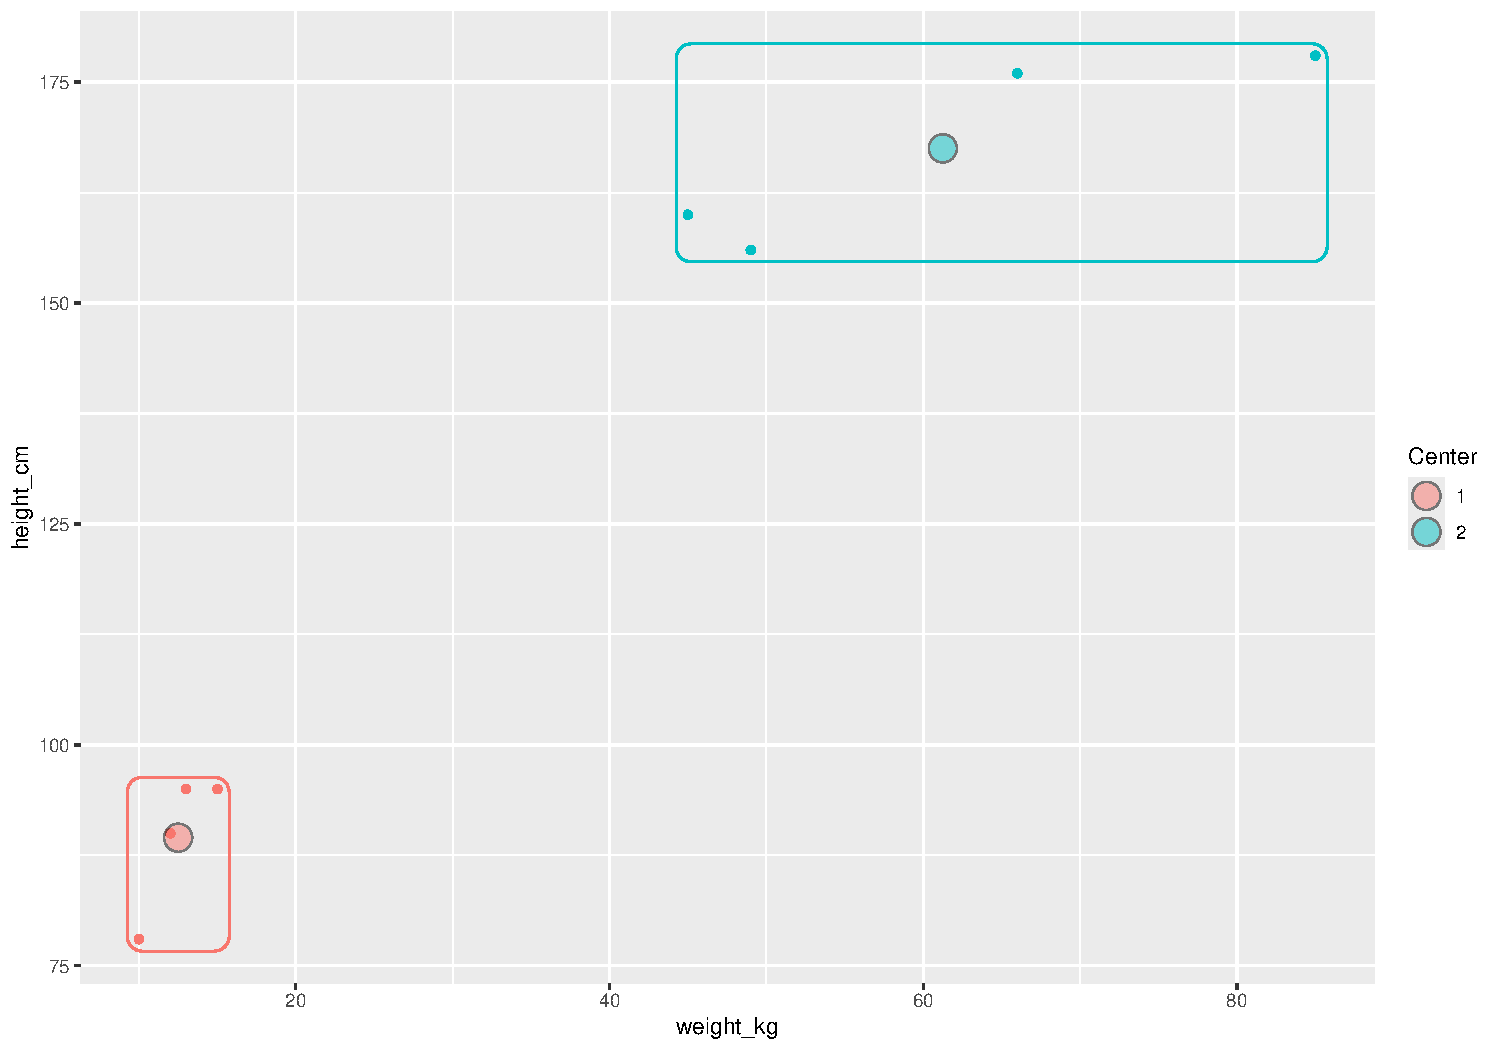
\includegraphics[width=0.6\textwidth,height=\textheight]{011_segmentation_clustering_files/figure-beamer/unnamed-chunk-30-1.pdf}
\end{center}
\end{frame}

\begin{frame}[fragile]{}
\phantomsection\label{section-43}
\begin{itemize}
\item
  K-means clustering example
  (\citeproc{ref-kaufman_finding_1990}{Kaufman and Rousseeuw 1990, 5})

  \begin{itemize}
  \tightlist
  \item
    Applying the
    \href{https://en.wikipedia.org/wiki/K-means_clustering}{\textbf{Hartigan-Wong
    algorithm}}
  \end{itemize}
\end{itemize}

\tiny

\begin{Shaded}
\begin{Highlighting}[]
\NormalTok{kaufman\_example\_kmeans }\OtherTok{\textless{}{-}}\NormalTok{ kaufman\_example }\SpecialCharTok{|\textgreater{}} 
  \FunctionTok{select}\NormalTok{(weight\_kg, height\_cm) }\SpecialCharTok{|\textgreater{}} 
  \FunctionTok{kmeans}\NormalTok{(}\AttributeTok{centers =} \DecValTok{2}\NormalTok{, }
         \AttributeTok{algorithm =} \StringTok{"Hartigan{-}Wong"}\NormalTok{) }\CommentTok{\# R uses this algorithm by default}

\NormalTok{kaufman\_example\_kmeans}
\end{Highlighting}
\end{Shaded}

\begin{verbatim}
K-means clustering with 2 clusters of sizes 4, 4

Cluster means:
  weight_kg height_cm
1     61.25     167.5
2     12.50      89.5

Clustering vector:
[1] 2 1 2 1 1 1 2 2

Within cluster sum of squares by cluster:
[1] 1371.75  206.00
 (between_SS / total_SS =  91.5 %)

Available components:

[1] "cluster"      "centers"      "totss"        "withinss"     "tot.withinss"
[6] "betweenss"    "size"         "iter"         "ifault"      
\end{verbatim}
\end{frame}

\begin{frame}[fragile]{}
\phantomsection\label{section-44}
\begin{itemize}
\tightlist
\item
  Extract clusters and assign them to observations
\end{itemize}

\tiny

\begin{Shaded}
\begin{Highlighting}[]
\NormalTok{kaufman\_example\_kmeans\_clusters }\OtherTok{\textless{}{-}}\NormalTok{ kaufman\_example }\SpecialCharTok{|\textgreater{}} 
  \FunctionTok{mutate}\NormalTok{(}\AttributeTok{cluster =}\NormalTok{ kaufman\_example\_kmeans}\SpecialCharTok{$}\NormalTok{cluster)}
\NormalTok{kaufman\_example\_kmeans\_clusters}
\end{Highlighting}
\end{Shaded}

\begin{verbatim}
# A tibble: 8 x 4
  name       weight_kg height_cm cluster
  <chr>          <dbl>     <dbl>   <int>
1 Ilan              15        95       2
2 Jacqueline        49       156       1
3 Kim               13        95       2
4 Lieve             45       160       1
5 Leon              85       178       1
6 Peter             66       176       1
7 Talia             12        90       2
8 Tina              10        78       2
\end{verbatim}
\end{frame}

\begin{frame}[fragile]{}
\phantomsection\label{section-45}
\begin{itemize}
\item
  Select a number of clusters, using \texttt{segmentation}, for example:
  4 clusters

  \begin{itemize}
  \item
    k-means only work with numerical data
  \item
    A possible solution is to transform categorical data into numerical
    data

    \begin{itemize}
    \tightlist
    \item
      If a variable is nominal only works if you have 2 categories
    \item
      If a variable is ordinal you assume that the notion of distance
      between them is constant or you need to specify integers to
      determine what distance is appropiate
    \item
      Also you need to scale the variables taking into account that you
      are mixing categorical and numerical variables
    \end{itemize}
  \end{itemize}
\end{itemize}
\end{frame}

\begin{frame}[fragile]{}
\phantomsection\label{section-46}
\begin{itemize}
\item
  Convert binary nominal data to numerical data

  \begin{itemize}
  \tightlist
  \item
    Only make sense when you have 2 categories
  \end{itemize}
\end{itemize}

\tiny

\begin{Shaded}
\begin{Highlighting}[]
\NormalTok{segmentation\_numeric }\OtherTok{\textless{}{-}}\NormalTok{ segmentation }\SpecialCharTok{|\textgreater{}} 
  \FunctionTok{mutate}\NormalTok{(}\AttributeTok{gender =} \FunctionTok{as.integer}\NormalTok{(gender),}
         \AttributeTok{ownHome =} \FunctionTok{as.integer}\NormalTok{(ownHome),}
         \AttributeTok{subscribe =} \FunctionTok{as.integer}\NormalTok{(subscribe))}

\NormalTok{segmentation\_numeric}
\end{Highlighting}
\end{Shaded}

\begin{verbatim}
# A tibble: 300 x 6
     age gender income  kids ownHome subscribe
   <dbl>  <int>  <dbl> <int>   <int>     <int>
 1  47.3      2 49483.     2       1         1
 2  31.4      2 35546.     1       2         1
 3  43.2      2 44169.     0       2         1
 4  37.3      1 81042.     1       1         1
 5  41.0      1 79353.     3       2         1
 6  43.0      2 58143.     4       2         1
 7  37.6      2 19282.     3       1         1
 8  28.5      2 47245.     0       1         1
 9  44.2      1 48333.     1       1         1
10  35.2      1 52568.     0       2         1
# i 290 more rows
\end{verbatim}
\end{frame}

\begin{frame}[fragile]{}
\phantomsection\label{section-47}
\begin{itemize}
\item
  Scale data to map each variable to a common scale

  \begin{itemize}
  \item
    We are going to scale each variable to \([0,1]\)

    \begin{itemize}
    \tightlist
    \item
      Use \texttt{across} and \texttt{rescale}
    \end{itemize}
  \end{itemize}
\end{itemize}

\tiny

\begin{Shaded}
\begin{Highlighting}[]
\NormalTok{segmentation\_numeric\_scale }\OtherTok{\textless{}{-}}\NormalTok{ segmentation\_numeric }\SpecialCharTok{|\textgreater{}} 
  \FunctionTok{mutate}\NormalTok{(}\FunctionTok{across}\NormalTok{(}\AttributeTok{.cols =}\NormalTok{ age}\SpecialCharTok{:}\NormalTok{subscribe,}
                \CommentTok{\# scales is a package that is }
                \CommentTok{\# installed with the tidyverse}
                \CommentTok{\# but it is not loaded automatically}
                \CommentTok{\# You can use a particular function of a package using the notation}
                \DocumentationTok{\#\# \textless{}package\textgreater{}::\textless{}function\textgreater{}}
                \AttributeTok{.fns =}\NormalTok{ scales}\SpecialCharTok{::}\NormalTok{rescale))}

\NormalTok{segmentation\_numeric\_scale }\SpecialCharTok{|\textgreater{}} \FunctionTok{head}\NormalTok{()}
\end{Highlighting}
\end{Shaded}

\begin{verbatim}
# A tibble: 6 x 6
    age gender income  kids ownHome subscribe
  <dbl>  <dbl>  <dbl> <dbl>   <dbl>     <dbl>
1 0.458      1  0.458 0.286       0         0
2 0.198      1  0.341 0.143       1         0
3 0.391      1  0.413 0           1         0
4 0.295      0  0.722 0.143       0         0
5 0.354      0  0.708 0.429       1         0
6 0.388      1  0.530 0.571       1         0
\end{verbatim}
\end{frame}

\begin{frame}[fragile]{}
\phantomsection\label{section-48}
\begin{itemize}
\item
  Apply k-means with \(k = 4\) and
  \href{https://en.wikipedia.org/wiki/K-means_clustering}{\textbf{Hartigan-Wong
  algorithm}}

  \begin{itemize}
  \tightlist
  \item
    k-means start with \(k = 4\) random centers so you need to fix this
    initial decision using \texttt{set.seed} if the clusters tend to
    change
  \end{itemize}
\end{itemize}

\tiny

\begin{Shaded}
\begin{Highlighting}[]
\FunctionTok{set.seed}\NormalTok{(}\AttributeTok{seed =} \DecValTok{1234}\NormalTok{)}

\NormalTok{segmentation\_numeric\_scale\_kmeans }\OtherTok{\textless{}{-}}\NormalTok{ segmentation\_numeric\_scale }\SpecialCharTok{|\textgreater{}} 
  \FunctionTok{kmeans}\NormalTok{(}\AttributeTok{centers =} \DecValTok{4}\NormalTok{, }
         \AttributeTok{algorithm =} \StringTok{"Hartigan{-}Wong"}\NormalTok{)}

\NormalTok{segmentation\_numeric\_scale\_kmeans }\SpecialCharTok{|\textgreater{}} \FunctionTok{str}\NormalTok{()}
\end{Highlighting}
\end{Shaded}

\begin{verbatim}
List of 9
 $ cluster     : int [1:300] 2 3 3 4 1 3 2 2 4 1 ...
 $ centers     : num [1:4, 1:6] 0.431 0.278 0.446 0.298 0 ...
  ..- attr(*, "dimnames")=List of 2
  .. ..$ : chr [1:4] "1" "2" "3" "4"
  .. ..$ : chr [1:6] "age" "gender" "income" "kids" ...
 $ totss       : num 218
 $ withinss    : num [1:4] 18.6 17.5 14.4 15.4
 $ tot.withinss: num 65.9
 $ betweenss   : num 152
 $ size        : int [1:4] 76 78 65 81
 $ iter        : int 3
 $ ifault      : int 0
 - attr(*, "class")= chr "kmeans"
\end{verbatim}
\end{frame}

\begin{frame}[fragile]{}
\phantomsection\label{section-49}
\begin{itemize}
\tightlist
\item
  Extract clusters and assign them to observations
\end{itemize}

\tiny

\begin{Shaded}
\begin{Highlighting}[]
\NormalTok{segmentation\_kmeans\_clusters }\OtherTok{\textless{}{-}}\NormalTok{ segmentation }\SpecialCharTok{|\textgreater{}} 
  \FunctionTok{mutate}\NormalTok{(}\AttributeTok{cluster =}\NormalTok{ segmentation\_numeric\_scale\_kmeans}\SpecialCharTok{$}\NormalTok{cluster)}

\NormalTok{segmentation\_kmeans\_clusters}
\end{Highlighting}
\end{Shaded}

\begin{verbatim}
# A tibble: 300 x 7
     age gender income  kids ownHome subscribe cluster
   <dbl> <fct>   <dbl> <int> <fct>   <fct>       <int>
 1  47.3 Male   49483.     2 ownNo   subNo           2
 2  31.4 Male   35546.     1 ownYes  subNo           3
 3  43.2 Male   44169.     0 ownYes  subNo           3
 4  37.3 Female 81042.     1 ownNo   subNo           4
 5  41.0 Female 79353.     3 ownYes  subNo           1
 6  43.0 Male   58143.     4 ownYes  subNo           3
 7  37.6 Male   19282.     3 ownNo   subNo           2
 8  28.5 Male   47245.     0 ownNo   subNo           2
 9  44.2 Female 48333.     1 ownNo   subNo           4
10  35.2 Female 52568.     0 ownYes  subNo           1
# i 290 more rows
\end{verbatim}
\end{frame}

\section{Acknowledgments}\label{acknowledgments}

\begin{frame}{}
\phantomsection\label{section-50}
\begin{itemize}
\item
  To my family that supports me
\item
  To the taxpayers of Colombia and the
  \href{https://www.umng.edu.co/estudiante}{\textbf{UMNG students}} who
  pay my salary
\item
  To the \href{https://www.business-science.io/}{\textbf{Business
  Science}} and \href{https://www.rfordatasci.com/}{\textbf{R4DS Online
  Learning}} communities where I learn
  \href{https://www.r-project.org/about.html}{\textbf{R}} and
  \href{https://www.python.org/about/}{\textbf{\(\pi\)-thon}}
\item
  To the \href{https://www.r-project.org/contributors.html}{\textbf{R
  Core Team}}, the creators of
  \href{https://posit.co/products/open-source/rstudio/}{\textbf{RStudio
  IDE}}, \href{https://quarto.org/}{\textbf{Quarto}} and the authors and
  maintainers of the packages
  \href{https://CRAN.R-project.org/package=tidyverse}{\textbf{tidyverse}},
  \href{https://CRAN.R-project.org/package=skimr}{\textbf{skimr}},
  \href{https://CRAN.R-project.org/package=latex2exp}{\textbf{latex2exp}},
  \href{https://CRAN.R-project.org/package=kableExtra}{\textbf{kableExtra}},
  \href{https://CRAN.R-project.org/package=cluster}{\textbf{cluster}}
  and
  \href{https://CRAN.R-project.org/package=tinytex}{\textbf{tinytex}}
  for allowing me to access these tools without paying for a license
\item
  To the \href{https://www.kernel.org/category/about.html}{\textbf{Linux
  kernel community}} for allowing me the possibility to use some
  \href{https://static.lwn.net/Distributions/}{\textbf{Linux
  distributions}} as my main
  \href{https://en.wikipedia.org/wiki/Operating_system}{\textbf{OS}}
  without paying for a license
\end{itemize}
\end{frame}

\section*{References}\label{references}
\addcontentsline{toc}{section}{References}

\begin{frame}[allowframebreaks]{References}
\phantomsection\label{refs}
\begin{CSLReferences}{1}{0}
\bibitem[\citeproctext]{ref-chapman_r_2019}
Chapman, Chris, and Elea McDonnell Feit. 2019. \emph{R {For} {Marketing}
{Research} and {Analytics}}. 2nd ed. 2019. Use {R}! Cham: Springer
International Publishing : Imprint: Springer.
\url{https://doi-org.ezproxy.umng.edu.co/10.1007/978-3-030-14316-9}.

\bibitem[\citeproctext]{ref-deza_encyclopedia_2016}
Deza, Michel Marie, and Elena Deza. 2016. \emph{Encyclopedia of
{Distances}}. Berlin, Heidelberg: Springer Berlin Heidelberg.
\url{https://doi.org/10.1007/978-3-662-52844-0}.

\bibitem[\citeproctext]{ref-kaufman_finding_1990}
Kaufman, Leonard, and Peter J. Rousseeuw. 1990. \emph{Finding {Groups}
in {Data}: {An} {Introduction} to {Cluster} {Analysis}}. 1st ed. Wiley
{Series} in {Probability} and {Statistics}. Wiley.
\url{https://doi.org/10.1002/9780470316801}.

\bibitem[\citeproctext]{ref-stevens_theory_1946}
Stevens, S. S. 1946. {``On the {Theory} of {Scales} of {Measurement}.''}
\emph{Science} 103 (2684): 677--80.
\url{https://doi.org/10.1126/science.103.2684.677}.

\end{CSLReferences}
\end{frame}




\end{document}
